\documentclass[11pt, xcolor=svgnames]{beamer}

\usepackage[T1]{fontenc}
\usepackage[english]{babel}
\usepackage[utf8x]{inputenc}
\usepackage{times}
\usepackage{sans}
\usepackage{graphicx}
\usepackage{longtable}
\usepackage{float}
\usepackage{wrapfig}
\usepackage{soul}
\usepackage{textcomp}
\usepackage{marvosym}
\usepackage{wasysym}
\usepackage{latexsym}
\usepackage{amssymb}
\usepackage{hyperref}
\usepackage{color}
\usepackage{verbatim}
\usepackage{url}
\usepackage{listings}
\lstset{
  basicstyle=\footnotesize\tt,        % the size of the fonts that are used for the code
  breakatwhitespace=false,         % sets if automatic breaks should only happen at whitespace
  breaklines=true,                 % sets automatic line breaking
  captionpos=b,                    % sets the caption-position to bottom
  extendedchars=true,              % lets you use non-ASCII characters; for 8-bits encodings only, does not work with UTF-8
  frame=single,                    % adds a frame around the code
  language=Java,                   % the language of the code
  keywordstyle=\bf,
  showspaces=false,                % show spaces everywhere adding particular underscores; it overrides 'showstringspaces'
  showstringspaces=false,          % underline spaces within strings only
  showtabs=false,                  % show tabs within strings adding particular underscores
  tabsize=2,                       % sets default tabsize to 2 spaces
  showstringspaces=false,
  keywordstyle=\color{blue},
  commentstyle=\color{green},
  stringstyle=\color{mauve}
}
%
% \lstset
% {
% language=SQL,
% basicstyle=\footnotesize,
% columns=fullflexible,
% keepspaces=true,
% breaklines=true,
% breakatwhitespace=true,
% tabsize=3,
% extendedchars=true,
% showstringspaces=false,
% keywordstyle=\color{blue},
% commentstyle=\color{dkgreen},
% stringstyle=\color{mauve}
% }

\definecolor{mauve}{rgb}{0.58,0,0.82}

\def\Tiny
{
\fontsize{5pt}{5pt}
\selectfont
}

\usepackage{tikz}
\usetikzlibrary{arrows}
\tikzstyle{block}=[draw opacity=0.7,line width=1.4cm]

\mode<presentation>
{
\usetheme{Warsaw}
\usefonttheme{serif}
\usecolortheme{whale}
\usefonttheme{structurebold}
\useoutertheme{infolines}

\setbeamercovered{transparent}
\setbeameroption{show notes}
\setbeamertemplate{blocks}[rounded][shadow=true]
\setbeamertemplate{navigation symbols}{}
\beamertemplateballitem
}

\tolerance=1000
\providecommand{\alert}[1]{\textbf{#1}}


\def\fig#1#2#3{
\begin{figure}[H]
\center
\includegraphics[#1]{#2}
\caption{#3\label{fig:#2}}
\end{figure}
}

%%%%%%%%%%%%%%%%%%%%%%%%%%%%%%%%%%%%%%%%%%%%%%%%%%%%%%%%%%%%%%%%%%%%%%%%%%%%%

\title {Introduction to Unit Testing}

\author[Daniel Rodriguez]{
  \textcolor{green!50!black}{Daniel Rodriguez}%\inst{1}
}
\institute[UAH]{University of Alcala}
\date{}

\setcounter{tocdepth}{1}

\begin{document}

\maketitle

\begin{frame}[fragile]{Outline}
  \tableofcontents
\end{frame}

\AtBeginSection
{
\begin{frame}
  \tableofcontents[currentsection]
\end{frame}
}

%%%%%%%%%%%%%%%%%%%%%%%%%%%%%%%%%%%%%%%%%%%%%%%%%%%%%%%%%%%%%%%%%%%%%%%%%%%%%%%
%%%%%%%%%%%%%%%%%%%%%%%%%%%%%%%%%%%%%%%%%%%%%%%%%%%%%%%%%%%%%%%%%%%%%%%%%%%%%%%

\section{Introduction}

%%%%%%%%%%%%%%%%%%%%%%%%%%%%%%%%%%%%%%%%%%%%%%%%%%%%%%%%%%%%%%%%%%%%%%%%%%%%%%%

\subsection{Definitions}

%%%%%%%%%%%%%%%%%%%%%%%%%%%%%%%%%%%%%%%%%%%%%%%%%%%%%%%%%%%%%%%%%%%%%%%%%%%%%%%

\begin{frame}{Testing}

  \begin{itemize}
   \item \alert{Error}: A human mistake.
   \item \alert{Fault}: The result of a mistake, evidenced in some development or maintenance product.
   \item \alert{Failure}: A departure from the system's required behaviour.
  \end{itemize}
  
  \begin{itemize}
   \item \alert{Fault identification (testing)}: Testing is the process of showing the presence of a software error. What fault caused the failure?
   \item \alert{Fault correction or removal (debugging)}: Debugging is the process of discovering the location of an error and its subsequent modification, i.e., changing the system to remove the fault.
  \end{itemize}
  
  \end{frame}


%%%%%%%%%%%%%%%%%%%%%%%%%%%%%%%%%%%%%%%%%%%%%%%%%%%%%%%%%%%%%%%%%%%%%%%%%%%%%%%

\begin{frame}[fragile]{Verification vs. Validation - IEEE Std610.12-1990}

\begin{itemize}
 \item \alert{Requirements Validation}. Process of checking that a document or piece of software accurately reflects the customer requirements - i.e. \\
 ARE WE BUILDING THE RIGHT SYSTEM?

\item \alert{Software Verification}. Process of ensuring that the product of one phase satisfies the product of a previous phase. sChecking that the software produced is a faithful implementation of the requirements specifiedAssessment of the quality of the implementation \\
ARE WE BUILDING IT RIGHT?
\end{itemize}

\end{frame}


%%%%%%%%%%%%%%%%%%%%%%%%%%%%%%%%%%%%%%%%%%%%%%%%%%%%%%%%%%%%%%%%%%%%%%%%%%%%%%%


\begin{frame}{Testing Process}

\begin{figure}
 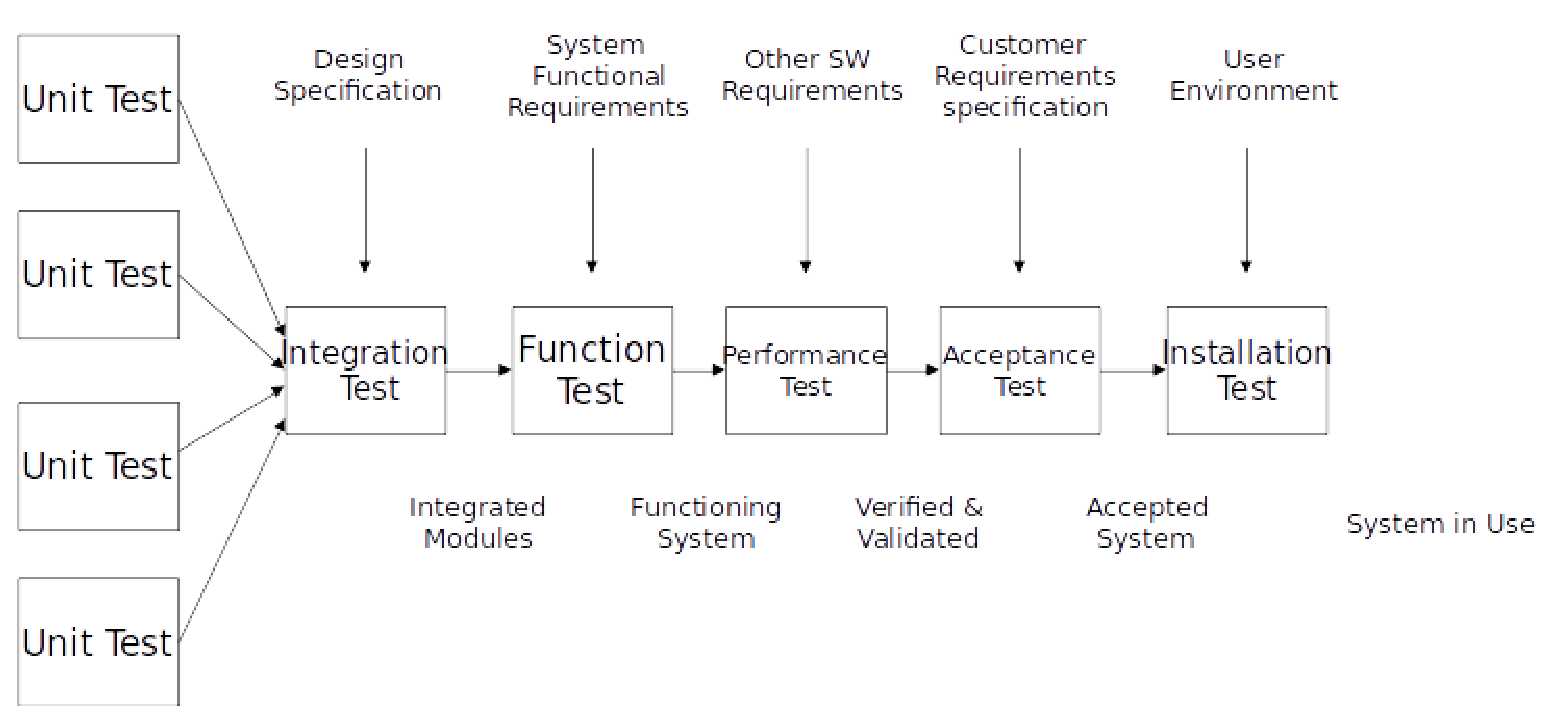
\includegraphics[width=300pt]{./figs/testing}
%\caption{}
\end{figure} 
\tiny{(Source: Plfeeger)}
\end{frame}


%%%%%%%%%%%%%%%%%%%%%%%%%%%%%%%%%%%%%%%%%%%%%%%%%%%%%%%%%%%%%%%%%%%%%%%%%%%%%%%


\section{Test Driven Development}


%%%%%%%%%%%%%%%%%%%%%%%%%%%%%%%%%%%%%%%%%%%%%%%%%%%%%%%%%%%%%%%%%%%%%%%%%%%%%%%


\begin{frame}{Fail, Pass, Refactor:  TDD Circle of life}

\begin{figure}
 \includegraphics[width=200pt]{./figs/tdd-circle-of-life.png}
%\caption{}
\end{figure} 


\tiny{Source:~\url{https://leantesting-wp.s3.amazonaws.com/resources/wp-content/uploads/2015/02/tdd-circle-of-life.png}}

\end{frame}


%%%%%%%%%%%%%%%%%%%%%%%%%%%%%%%%%%%%%%%%%%%%%%%%%%%%%%%%%%%%%%%%%%%%%%%%%%%%%%%


\begin{frame}{Fail, Pass, Refactor:  TDD Circle of life}

\begin{block}{TDD Life-cycle}
	\begin{enumerate}
		\item Identify functionality to include
		\item Write failing test
		\item Make it compile as quickly as possible
		\item Make it pass a quickly as possible
		\item Refactor: remove duplication while maintaining 100\% pass rate
		\item Repeat as required
	\end{enumerate}
\end{block}

\end{frame}

%%%%%%%%%%%%%%%%%%%%%%%%%%%%%%%%%%%%%%%%%%%%%%%%%%%%%%%%%%%%%%%%%%%%%%%%%%%%%%%

\section{Assertions}

%%%%%%%%%%%%%%%%%%%%%%%%%%%%%%%%%%%%%%%%%%%%%%%%%%%%%%%%%%%%%%%%%%%%%%%%%%%%%%%

\begin{frame}{What are Assertions?}

  An \alert{assertion} specifies a constraint over some state of computation. If it evaluates to false, it implies there exists an incorrect state in the program.
  
  Assertions: 
  
  \begin{itemize}
    \item can test whether the execution state is consistent at the point of examination.
    \item are predicates involving the state variables of a program in execution.
    \item are embedded in the program text.
  \end{itemize}
  
  Assertions are part of most programming languages.
  
  \end{frame}


%%%%%%%%%%%%%%%%%%%%%%%%%%%%%%%%%%%%%%%%%%%%%%%%%%%%%%%%%%%%%%%%%%%%%%%%%%%%%%%

\begin{frame}{Assertions: History}


Hoare and Floyd started in the 60s (Hoare logic) the formal verification of programs. They introduced the concept of \emph{preconditions}, \emph{postconditions} and \emph{invariants}.

A triple describes how the execution of a piece of code changes the state of the computation:

  $[\{P\}C\{Q\}]$

\noindent where $P$ and $Q$ are assertions and $C$ is code.

\begin{itemize}
	\item $P$ precondition 
	\item $Q$ postcondition
\end{itemize}

In other words, a program behaviour can be verified using preconditions, postconditions and invariants.


\end{frame}

%%%%%%%%%%%%%%%%%%%%%%%%%%%%%%%%%%%%%%%%%%%%%%%%%%%%%%%%%%%%%%%%%%%%%%%%%%%%%%%

\begin{frame}[fragile]{Assertions in Java}

  Assertions in Java are written as:

  \begin{lstlisting}[language=JAVA,basicstyle=\small]
  assert expression;
  \end{lstlisting}
  
  \texttt{assert} is a Java keyword and \texttt{expression} is any Boolean expression. When evaluated to \texttt{false}, an exception, \texttt{AssertionError}, will be raised. 
  
  They can also provide information for developers:
  
  \begin{lstlisting}[language=JAVA,basicstyle=\small]
  assert expression1 : expression2;
  \end{lstlisting}

\end{frame}

%%%%%%%%%%%%%%%%%%%%%%%%%%%%%%%%%%%%%%%%%%%%%%%%%%%%%%%%%%%%%%%%%%%%%%%%%%%%%%%

\begin{frame}[fragile]{\texttt{Assert} Example}

\begin{lstlisting}[language=JAVA,basicstyle=\scriptsize]
  public double avgMarks(double[] marks){
 	// Pre-condition
	assert marks.length > 0 : "Array is empty!";
   	double avg = 0;
   	for (int i = 0 ; i < marks.length; i++){
	     //Invariant	
   	     assert marks[i] >= 0 && marks[i] <= 10 : "Mark is not valid!";
   	     avg += marks[i];
   	}
   	return avg/marks.length;
   }
\end{lstlisting}

\end{frame}



%%%%%%%%%%%%%%%%%%%%%%%%%%%%%%%%%%%%%%%%%%%%%%%%%%%%%%%%%%%%%%%%%%%%%%%%%%%%%%%

\begin{frame}[fragile]{\texttt{Assert} example}

\begin{lstlisting}[language=JAVA,basicstyle=\scriptsize]
public class AssertionExample {
  public double avgMarks(double[] marks){
   	assert marks.length > 0 : "Array is empty!";
   	double avg = 0;
   	for (int i = 0; i < marks.length; i++) {
   	     assert marks[i] >= 0 && marks[i] <= 10 : "Mark is not valid!";
   	     avg += marks[i];
   	}
   	return avg/marks.length;
   }

  public static void main(String args[]){
   	AssertionExample e = new AssertionExample();
   	double[] marks = {10, 5, 11, 3, 2, 7.5};
   	System.out.println(e.avgMarks(marks));
   	marks = new double[0];
   	System.out.println(e.avgMarks(marks));
   }
}
\end{lstlisting}


\end{frame}



%%%%%%%%%%%%%%%%%%%%%%%%%%%%%%%%%%%%%%%%%%%%%%%%%%%%%%%%%%%%%%%%%%%%%%%%%%%%%

\begin{frame}[fragile]{\texttt{Assert} example}

When assertions are evaluated when enabled, i.e., with the VM options \texttt{-enableassertions} or \texttt{-ea}:

\begin{lstlisting}[language=JAVA,basicstyle=\scriptsize]
$java -ea AssertionExample
\end{lstlisting}

\begin{center}
 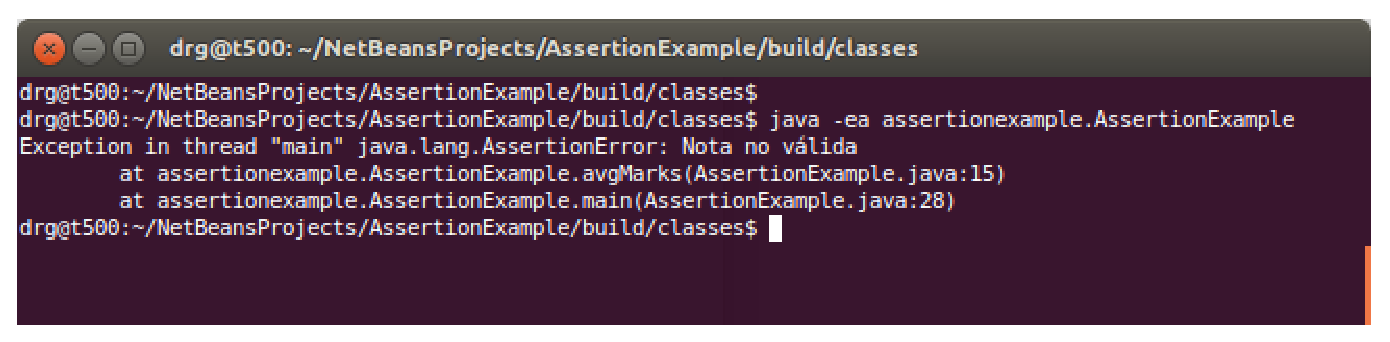
\includegraphics[width=\columnwidth]{./figs/assertionsExeption}
\end{center}

%assertionsExeption 

Otherwise, it will run normally as assertions are designed to be run during the testing phase or debugging.

\end{frame}

%%%%%%%%%%%%%%%%%%%%%%%%%%%%%%%%%%%%%%%%%%%%%%%%%%%%%%%%%%%%%%%%%%%%%%%%%%%%%

\begin{frame}[fragile]{Assertions vs Exceptions}

Assertions are designed to check the program's correctness, i.e, as \emph{preconditions}, \emph{postconditions} or \emph{invariants}.

Assertions can be used to verify the state of a program but should NOT be used to:

\begin{itemize}
\item Validate arguments of public methods
\item Substitute the \textbf{exception handling} mechanims of a programming language
\item Modify values of attributes or objects
\item Be used in production code (assertions abruptly stop the execution of a program)
\end{itemize}

Exception handling is the process of responding to the occurrence of exceptions (usually in a graceful manner so that the execution is not interrupted). In Java, this is carried out with \texttt{try() ... catch() ... finally} statements.

Although most programming languages provide assertions, unit testing is usually carried out with frameworks such as jUnit (Java) or pyest (Python). 

\end{frame}


%%%%%%%%%%%%%%%%%%%%%%%%%%%%%%%%%%%%%%%%%%%%%%%%%%%%%%%%%%%%%%%%%%%%%%%%%%%%%
%%%%%%%%%%%%%%%%%%%%%%%%%%%%%%%%%%%%%%%%%%%%%%%%%%%%%%%%%%%%%%%%%%% JUnit %%%

\section{JUnit}

%%%%%%%%%%%%%%%%%%%%%%%%%%%%%%%%%%%%%%%%%%%%%%%%%%%%%%%%%%%%%%%%%%%%%%%%%%%%%%%

\begin{frame}{What is JUnit}

\begin{block}{}
  \centering \url{https://www.junit.org/}
\end{block}

\begin{itemize}
    \item JUnit is the most popular open source unit testing framework in Java.
    \item JUnit is a regression testing framework.
    \item Created in 1997 by Erich Gamma and Kent Beck.
    \item Simple framework with a small learning curve.
    \item Tests can be automated (facilitates regression testing). It allow us to aggregate tests via test suites.
    \item \textit{De facto} standard, integrated with Ant, Maven, Gradle, etc. Typically run with continuous integration testing tools. 
    %\item \texttt{\url{https://www.junit.org/}}
\end{itemize}




\begin{block}{}
  ''Never in the field of software development have so many owed so much to so few lines of code'' (Martin Fowler)
\end{block}

\end{frame}



% %%%%%%%%%%%%%%%%%%%%%%%%%%%%%%%%%%%%%%%%%%%%%%%%%%%%%%%%%%%%%%%%%%%%%%%%%%%%%

% \begin{frame}{JUnit 3 - (Obsolete)}

% There are still a lot of test cases and frameworks that use JUnit 3 or 4. We briefly describe how to do test cases with JUnit 3 and 4 to understand them (But we will only work with JUnit 5).

% JUnit 3 was based on inheritance and name conventions (it is common to still use them). With JUnit 3, we needed to create test classes as follows:

% \begin{itemize}
%   \item Add \texttt{JUnit3<version>.jar} to the \texttt{classpath}
%   \item Create a subclass extending the \texttt{TestCase} class provided by JUnit
%   \item Define one or more public \texttt{testXXX()} methods in the subclass.
%   \begin{itemize}
%     \item Write assert methods inside the \texttt{testXXX()} methods to compare actual results (obtained from the CUT) with the expected results (the oracle)
%   \end{itemize}
%   \item Optionally, define \texttt{main()} to run the TestCase in batch mode (test runner)
% \end{itemize}


% \end{frame}

% %%%%%%%%%%%%%%%%%%%%%%%%%%%%%%%%%%%%%%%%%%%%%%%%%%%%%%%%%%%%%%%%%%%%%%%%%%%%%

% \begin{frame}[fragile]{JUnit 3 (Obsolete) - Architecture }

% Main classes: 

% \begin{center}
%   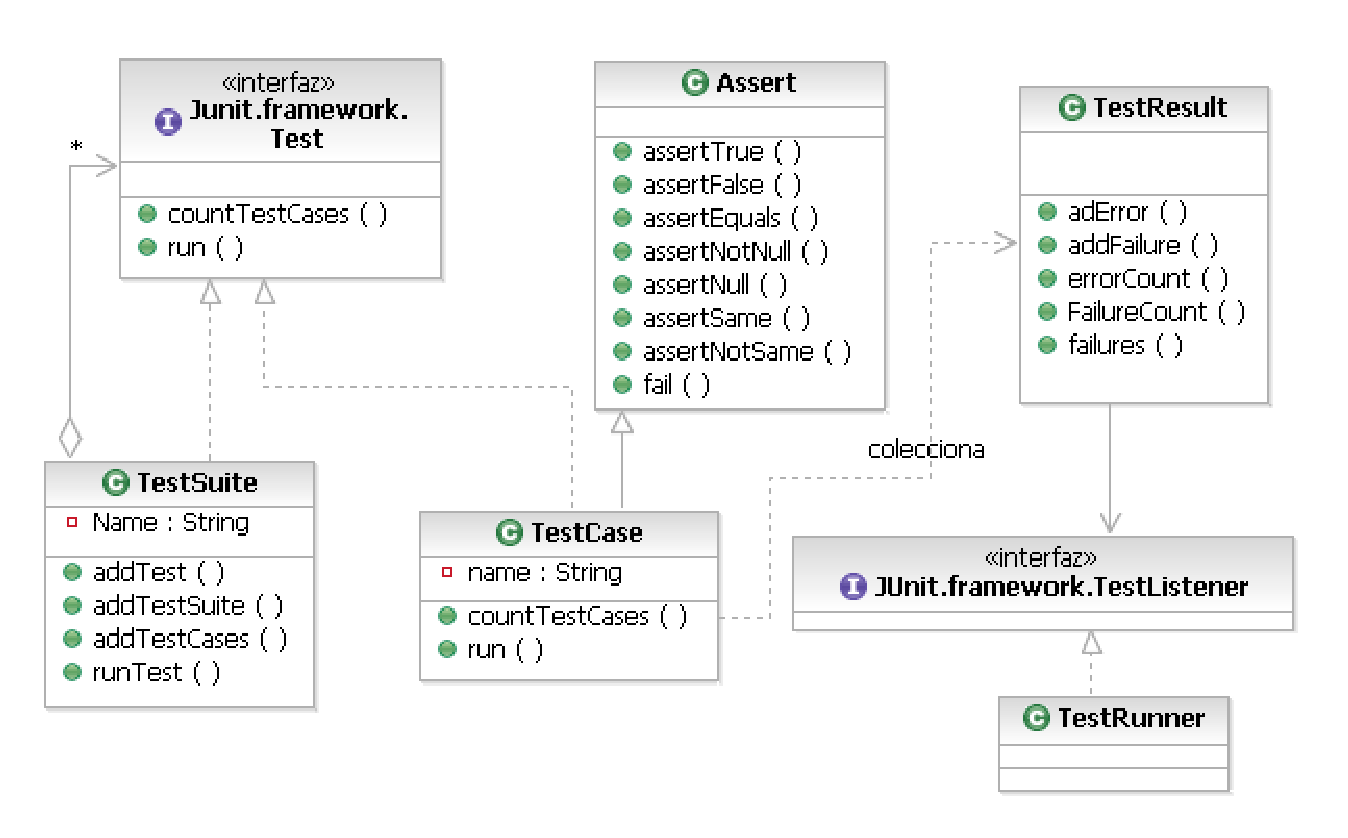
\includegraphics[width=300pt]{./figs/UMLJUnit3}
% \end{center}
 
% \end{frame}

% %%%%%%%%%%%%%%%%%%%%%%%%%%%%%%%%%%%%%%%%%%%%%%%%%%%%%%%%%%%%%%%%%%%%%%%%%%%%%

% \begin{frame}[fragile]{JUnit3 (Obsolete) Minimal example}

% \begin{lstlisting}[language=Java,basicstyle=\scriptsize]
% import junit.framework.TestCase;

% public class MinimalTest extends TestCase {

%   public MinimalTest(String name) {
%     super(name);
%   }
%   // Test method
%   public void testCUT () {
%     int expected = 2; //expected result
%     int actual = new CUT(); //get the actual result from CUT
%     assertTrue(actual, expected);
%   }
%   // Not needed, it's possible to use Test runner
%   public static void main(String[] args){
%     junit.textui.TestRunner.run(MinimalTest.class);
%   }
% }
% \end{lstlisting}

% \end{frame}

% %%%%%%%%%%%%%%%%%%%%%%%%%%%%%%%%%%%%%%%%%%%%%%%%%%%%%%%%%%%%%%%%%%%%%%%%%%%%%

% % \begin{frame}[fragile]{JUnit 3 (Obsolete) - Characteristics}

% % Fixtures are used to initialize and release common test data, this is done with \texttt{setUp()} and \texttt{tearDown()}.

% % \begin{itemize}
% %     \item \texttt{setUp()} is used for setting things up before \textbf{each} test
% %     \item \texttt{tearDown()} for tearing things down after \textbf{each} test
% % \end{itemize}
  
% % Suites can contain multiple test cases: \texttt{addTest(Test test)}

% % \begin{lstlisting}[language=JAVA,basicstyle=\scriptsize]
% %   public static void main (String [] args){
% %     junit.textui.TestRunner.run (suite ());
% %   }
% %   // TestSuite implements Test interface
% %   public static Test suite() {
% %     TestSuite suite = new TestSuite("AllTests");
% %     suite.addTest(new TestSuite(FloatTest.class));
% %     suite.addTest(new TestSuite(BoolTest.class));
% %     return suite;
% %   }
% %   public void testAllTests () throws Exception{
% %       assertTrue (suite != null);
% %   }
% % \end{lstlisting}

% % \end{frame}


%%%%%%%%%%%%%%%%%%%%%%%%%%%%%%%%%%%%%%%%%%%%%%%%%%%%%%%%%%%%%%%%%%%%%%%%%%%%%

\subsection{JUnit 4}

%%%%%%%%%%%%%%%%%%%%%%%%%%%%%%%%%%%%%%%%%%%%%%%%%%%%%%%%%%%%%%%%%%%%%%%%%%%%%

\begin{frame}{JUnit 4}

JUnit 4 took advantage of imports and annotations included in JDK 5+.
\begin{itemize}
  \item Static imports. It allow us to make use of static variables and methods from other classes without qualifying them (name the class).
  \item Annotations 
  \begin{itemize}
    \item Annotations are metadata that provide information to the compiler (or other tools)
    \item JUnit 4 works with annotations instead of extending classes. There is no need for naming conventions as in previous versions but those naming patterns are still used. 
  \end{itemize}
  \item JUnit4 also improved the functionality with annotations
  \begin{itemize}
    \item Timeouts: \texttt{@Test(timeout=1000)}...
    \item Testing exceptions: \texttt{@Test(expected=DBConnectException.class)} 
    \item Ignore a test: \texttt{@Ignore("Ignore the following test for now")}
  \end{itemize}
\end{itemize}

\end{frame}


%%%%%%%%%%%%%%%%%%%%%%%%%%%%%%%%%%%%%%%%%%%%%%%%%%%%%%%%%%%%%%%%%%%%%%%%%%%%%

\begin{frame}{Junit 4 -- Annotations}

\begin{itemize}
  \item \texttt{@Before} A method marked with \texttt{@Before} will be run before every test method. It is used to prepare the tests environment.
  \item \texttt{@After}
  \item \texttt{@Test} Identifies a test method.
  \item \texttt{@Ignore} The method under test will be ignored (to disable some tests which we do not want to repeat)
  \item \texttt{@AfterClass} Run only once after all test methods
  \item \texttt{@BeforeClass}
  \end{itemize}
\end{frame}

%%%%%%%%%%%%%%%%%%%%%%%%%%%%%%%%%%%%%%%%%%%%%%%%%%%%%%%%%%%%%%%%%%%%%%%%%%%%%

\subsection{JUnit 5}

%%%%%%%%%%%%%%%%%%%%%%%%%%%%%%%%%%%%%%%%%%%%%%%%%%%%%%%%%%%%%%%%%%%%%%%%%%%%%

\begin{frame}{Junit 5 -- Annotations}

  \begin{itemize}
    \item \texttt{@BeforeEach} A method marked with \texttt{@BeforeEach} will be run before every test method. It is used to prepare the tests environment.
    \item \texttt{@AfterEach} It will be run after every test method.
    \item \texttt{@Test} Identifies a test method.
    \item \texttt{@Ignore} The method under test will be ignored (to disable some tests which we do not want to repeat)
    \item \texttt{@AfterAll} Run only once after all test methods
    \item \texttt{@BeforeAll} Run only once before all test methods
    \end{itemize}
  \end{frame}
 

%%%%%%%%%%%%%%%%%%%%%%%%%%%%%%%%%%%%%%%%%%%%%%%%%%%%%%%%%%%%%%%%%%%%%%%%%%%%%

\begin{frame}{Junit 5 -- Assert methods}

Assert methods are used to comparison between an expected value and an actual value to determine the success or failure of a test.
  
      \begin{itemize}
        \item \texttt{assertCONDITION(...)}
        \item \texttt{assertCONDITION(String message,...)} - The message is displayed when the assert method fails
      \end{itemize}
  
For example:

      \begin{itemize}
        \item \texttt{assertEquals(<> expected, <> actual)}
        \item \texttt{assertSame(...)} 
        \item \texttt{assertFalse(boolean condition)}
        \item \texttt{assertTrue(boolean condition)}
        %\item \texttt{assertNull(...)}
        %\item \texttt{assertNotNull(...)}
        \item Etc.
      \end{itemize}

Further information in the API: \texttt{org.junit.jupiter.api.Assertions}

%\url{https://junit.org/junit5/}
  
\end{frame}

%%%%%%%%%%%%%%%%%%%%%%%%%%%%%%%%%%%%%%%%%%%%%%%%%%%%%%%%%%%%%%%%%%%%%%%%%%%%%

\begin{frame}{Junit 5 -- New functionality I}

  \begin{itemize}
    \item Custom display names - The \texttt{@DisplayName} annotation allows us to provide custom display names for test classes and methods, which can include spaces, special characters, and emojis.
  
    \item Nested test classes - Non-static nested classes (i.e., inner classes) can serve as \texttt{@Nested} test classes for logical grouping of test cases. 
  
    \item Tagging and filtering - It is possible to tag test classes and test methods with your identifiers using the \texttt{@Tag} annotation. 
  
    \item Meta-annotations and composed annotations - This allows us to create a custom composed annotation that will inherit the semantics of its meta-annotations.
  \end{itemize}

\end{frame}

%%%%%%%%%%%%%%%%%%%%%%%%%%%%%%%%%%%%%%%%%%%%%%%%%%%%%%%%%%%%%%%%%%%%%%%%%%%%%

\begin{frame}{Junit 5 -- New functionality II}

  \begin{itemize}
    \item Dynamic tests - JUnit Jupiter introduces dynamic tests which are generated at runtime by a factory method annotated with the \texttt{@TestFactory} annotation.
  
    \item Repeated tests - Tests can be repeated a specified number of times by annotating the test method with the \texttt{@RepeatedTest} annotation.
  
    \item Parameterized tests - A test can be run multiple times with different arguments by annotating the test method with the \texttt{@ParameterizedTest} annotation.
    % and declaring at least one source to provide the arguments. 
  \end{itemize}

\end{frame}

%%%%%%%%%%%%%%%%%%%%%%%%%%%%%%%%%%%%%%%%%%%%%%%%%%%%%%%%%%%%%%%%%%%%%%%%%%%%%

\section{First Example}

%%%%%%%%%%%%%%%%%%%%%%%%%%%%%%%%%%%%%%%%%%%%%%%%%%%%%%%%%%%%%%%%%%%%%%%%%%%%%


\begin{frame}[fragile]{\texttt{ComplexNumber} Class -- Class Under Test (CUT)}

  We will use the \texttt{ComplexNumber} class as example, which will later be used to calculate quadratic equations.
  
  The structure of the \texttt{ComplexNumber} class is as follows:
  
  \begin{center}
   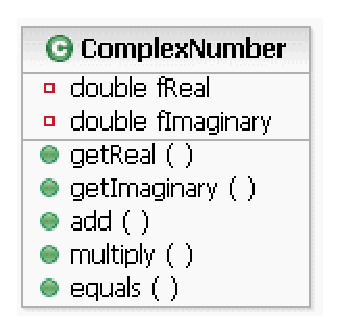
\includegraphics[width=75pt]{./figs/ComplexNumber}
  \end{center}
  
  The operations are as follows:
  
  \begin{itemize}
   \item Addition: $(a,b)+(c,d)=(a+c)+(b+d)i$
   \item Multiplication: $(a,b)\cdot(c,d)=(ac-bd) + (ad+cb)i$
   \item Equality: $(a,b)=(c,d) \Leftrightarrow a=c \wedge b=d$
  \end{itemize}
  
  \end{frame}


%%%%%%%%%%%%%%%%%%%%%%%%%%%%%%%%%%%%%%%%%%%%%%%%%%%%%%%%%%%%%%%%%%%%%%%%%%%%%


\begin{frame}[fragile]{\texttt{ComplexNumber} class -- CUT I}


\begin{lstlisting}[language=Java,basicstyle=\scriptsize]
public class ComplexNumber {
    private double fReal;
    private double fImaginary;

  public ComplexNumber(double re, double im) {
    fReal = re;
    fImaginary = im;
  }

  public double getReal() {
    return fReal;
  }

  public double getImaginary() {
    return fImaginary;
  }
}

public ComplexNumber add(ComplexNumber c) {
  return new ComplexNumber(getReal() + c.getReal(), 
                           getImaginary() + c.getImaginary());
}
\end{lstlisting}

\end{frame}

%%%%%%%%%%%%%%%%%%%%%%%%%%%%%%%%%%%%%%%%%%%%%%%%%%%%%%%%%%%%%%%%%%%%%%%%%%%%%

\begin{frame}[fragile]{\texttt{ComplexNumber} class -- CUT II}

\begin{lstlisting}[language=Java,basicstyle=\scriptsize]
public ComplexNumber multiply(ComplexNumber c) {
  double re = getReal() * c.getReal() - getImaginary() * c.getImaginary();
  double im = getImaginary() * c.getReal() + getReal() * c.getImaginary();
  return new ComplexNumber(re, im);
}

@Override
public boolean equals(Object anObject) {
  if (anObject instanceof ComplexNumber) {
    ComplexNumber c = (ComplexNumber) anObject;
    return ((c.getReal() == getReal()) && 
            (c.getImaginary() == getImaginary()));
  } else
    return false;
  }
}
\end{lstlisting}

\end{frame}


% %%%%%%%%%%%%%%%%%%%%%%%%%%%%%%%%%%%%%%%%%%%%%%%%%%%%%%%%%%%%%%%%%%%%%%%%%%%%%
% %%%%%%%%%%%%%%%%%%%%%%%%%%%%%%%%%%%%%%%%%%%%%%%%%%%%%%%%%%%%%%%%%%%%%%%%%%%%%

% % \subsection{JUnit in Eclipse}

% %%%%%%%%%%%%%%%%%%%%%%%%%%%%%%%%%%%%%%%%%%%%%%%%%%%%%%%%%%%%%%%%%%%%%%%%%%%%%

% % \begin{frame}{MoreUnit}
% %
% %MoreUnit makes unit testing in Eclipse a bit easier.
% %  
% %To install MoreUnit in Eclipse, select Help \textgreater Eclipse Marketplace
% %  
% %  \begin{center}
% %    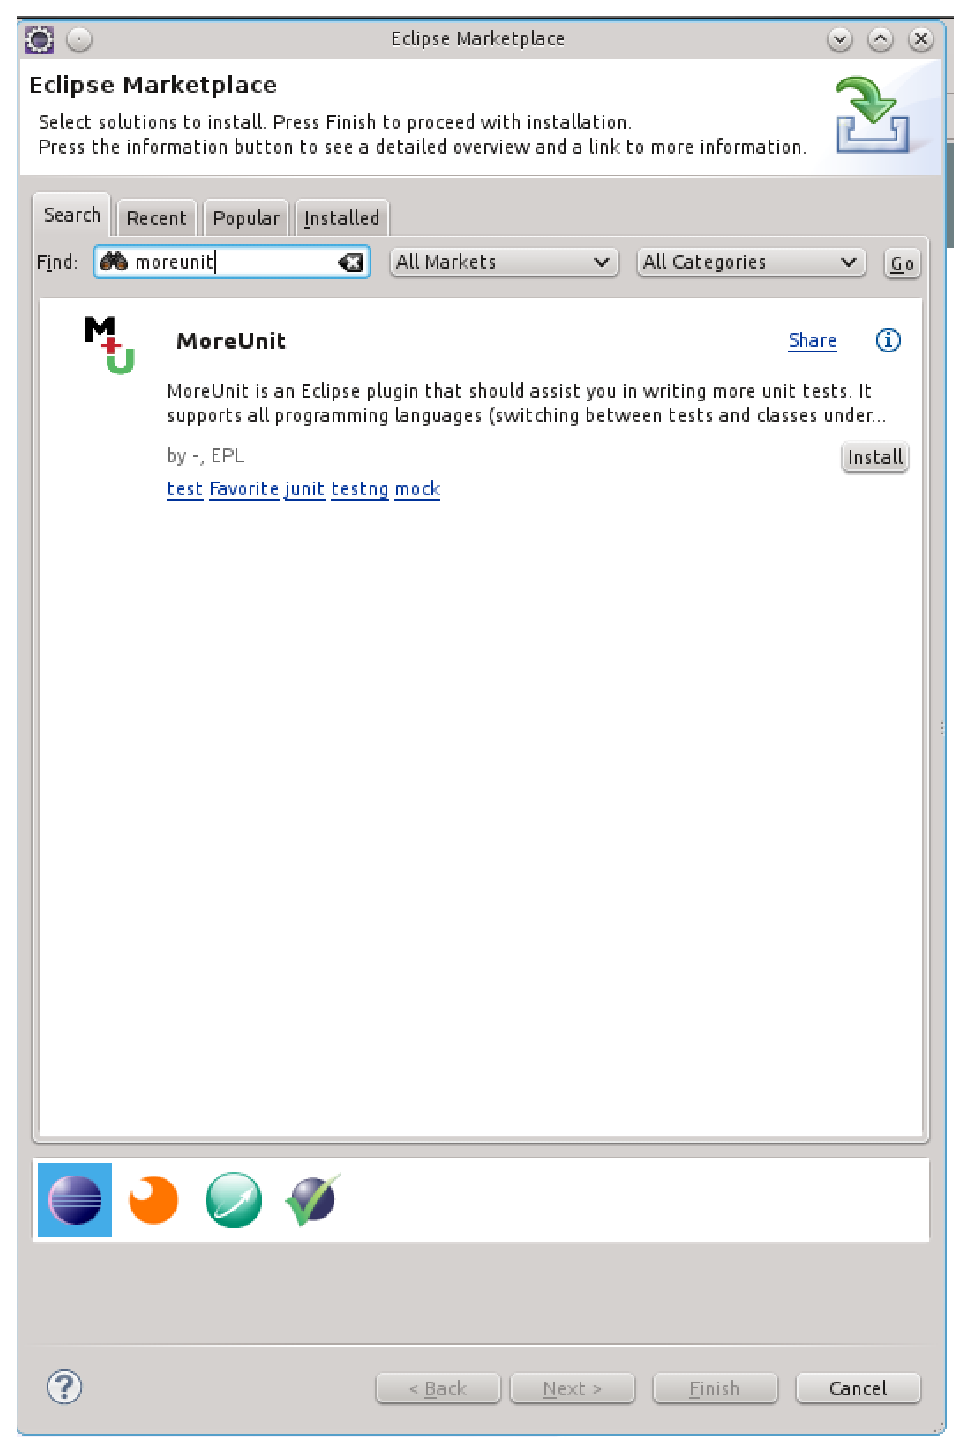
\includegraphics[width=100pt]{./figs/market}
% %  \end{center}
% %  
% %  \texttt{Next} and then \texttt{Finish} (restart Eclipse)
% %
% %    More about MoreUnit: \texttt{https://moreunit.github.io/MoreUnit-Eclipse/ }
% %\end{frame}


% %%%%%%%%%%%%%%%%%%%%%%%%%%%%%%%%%%%%%%%%%%%%%%%%%%%%%%%%%%%%%%%%%%%%%%%%%%%%%

% %\begin{frame}
% %
% %Configure MoreUnit Source folder
% %
% %  Import the JUnit library and create a source folder for the tests in each project which you want to have unit tests. Click \texttt{Window} \textgreater \texttt{Preferences}:
% %
% %    \begin{center}
% %    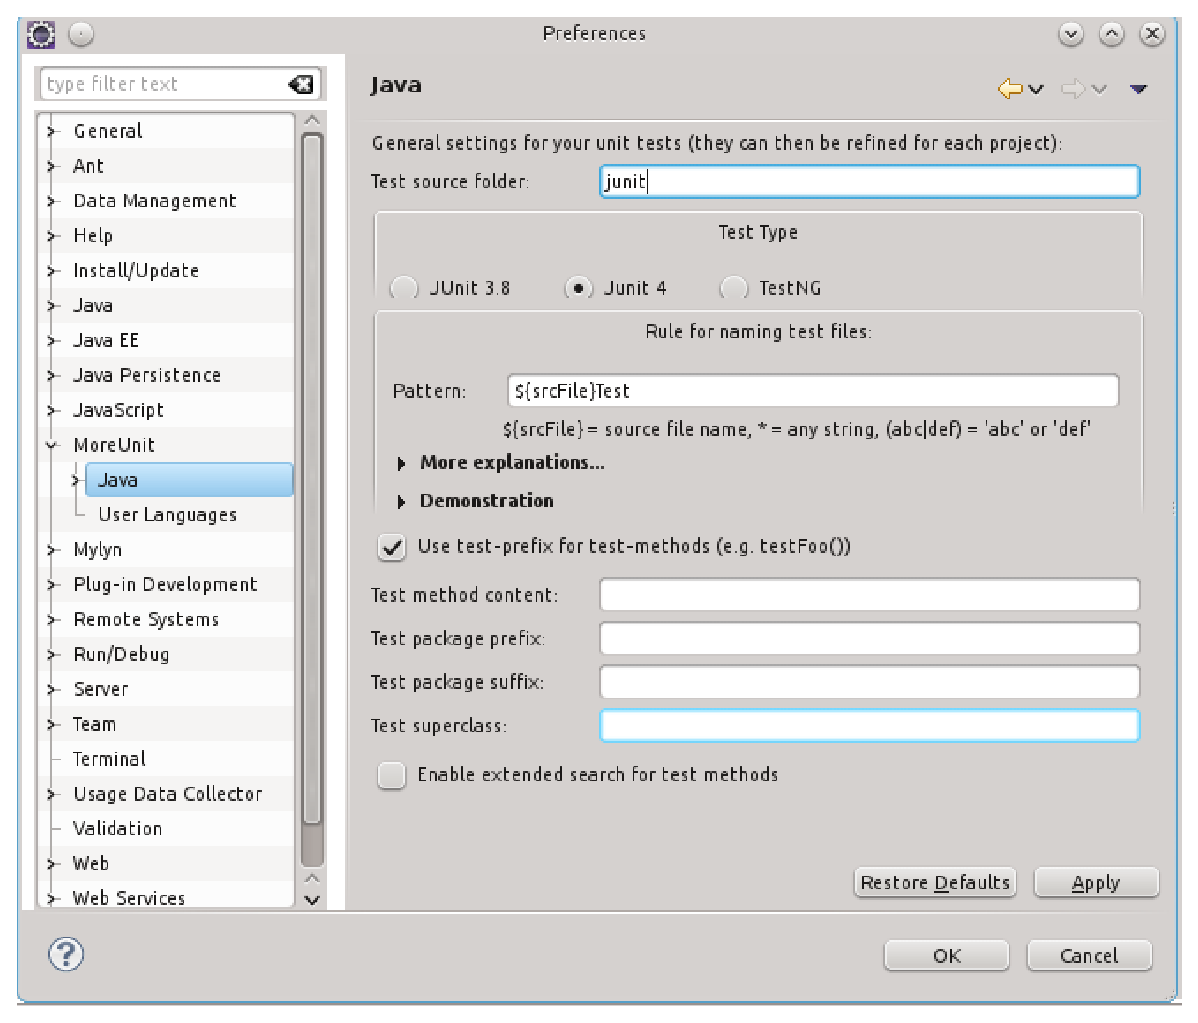
\includegraphics[width=205pt]{./figs/config}                                            
% %    \end{center}
% %      
% %    Set \texttt{Test} as Source Folder.
% %
% %\end{frame}

% %%%%%%%%%%%%%%%%%%%%%%%%%%%%%%%%%%%%%%%%%%%%%%%%%%%%%%%%%%%%%%%%%%%%%%%%%%%%%

% %\begin{frame}
% %    Starting with MoreUnit. With a new Java Project:
% %    \begin{enumerate}
% %      \item Open the project properties
% %      \item Click on \emph{Java Build Path}
% %      \item Select the \emph{Libraries} tab
% %      \item Click the \emph{Add Library} button
% %      \item Choose JUnit
% %    \end{enumerate}
% %\end{frame}

% %%%%%%%%%%%%%%%%%%%%%%%%%%%%%%%%%%%%%%%%%%%%%%%%%%%%%%%%%%%%%%%%%%%%%%%%%%%%%

% %\begin{frame}
% %     In your Java Project, create a new source folder called 'test', in your folder right click and select \texttt{New} \textgreater \texttt{Source Folder}.
% %
% %    \begin{center}
% %      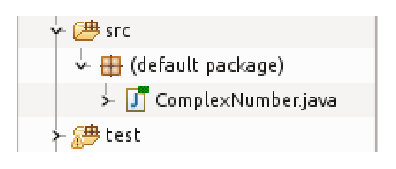
\includegraphics[width=150pt]{./figs/folder}
% %    \end{center}
% %
% %\end{frame}

% % %%%%%%%%%%%%%%%%%%%%%%%%%%%%%%%%%%%%%%%%%%%%%%%%%%%%%%%%%%%%%%%%%%%%%%%%%%%%%

% %\begin{frame}

% %In the class with the code you have to do right click and select MoreUnit menu \textgreater Jump to test/Member under test.

% %\begin{center}
% %  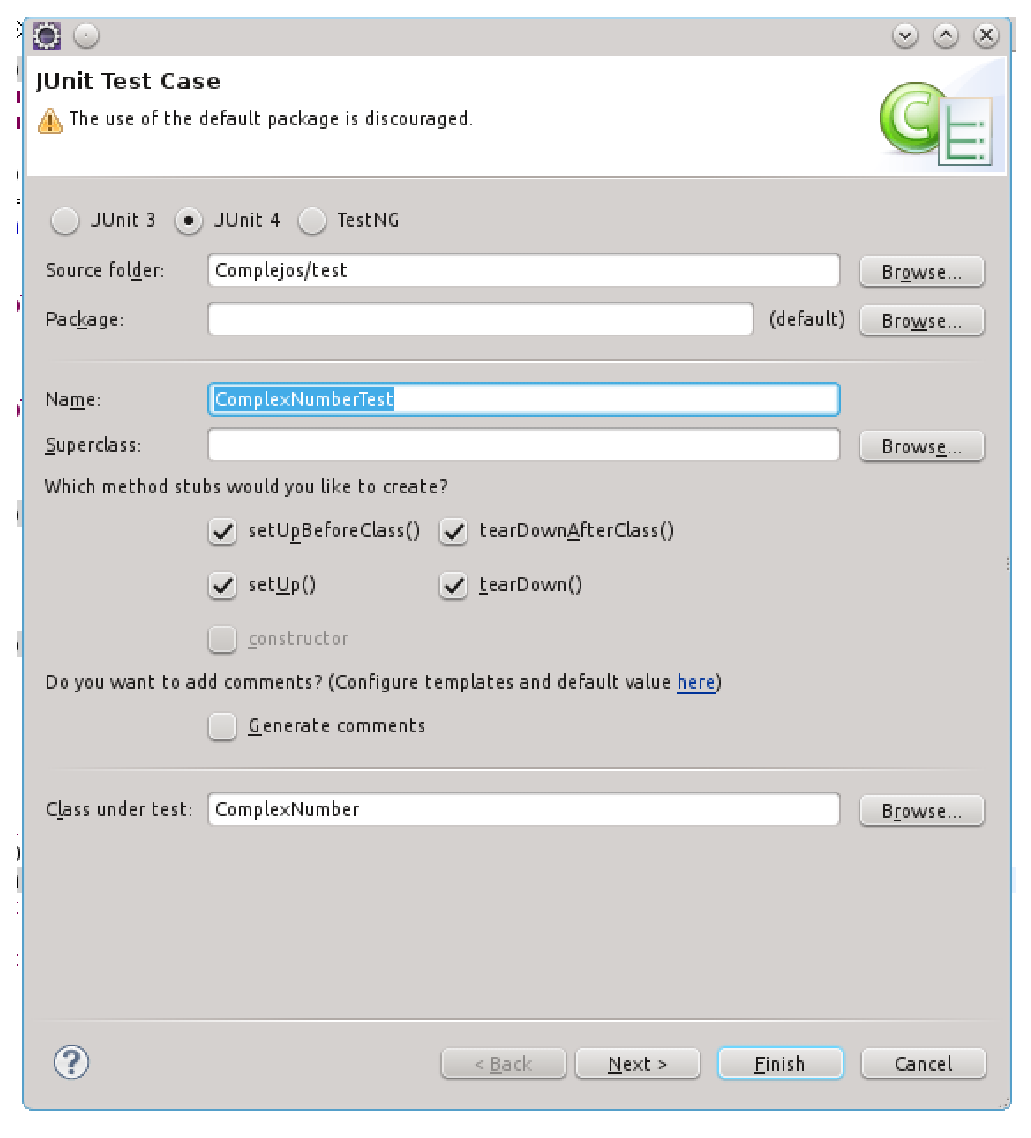
\includegraphics[width=150pt]{./figs/Unitmenu}
% %\end{center}
% %
% %\end{frame}

%%%%%%%%%%%%%%%%%%%%%%%%%%%%%%%%%%%%%%%%%%%%%%%%%%%%%%%%%%%%%%%%%%%%%%%%%%%%

\begin{frame}[fragile]{Fixtures}

Now you can view your test class in the test source folder. Extract from test class:

\begin{center}
\begin{lstlisting}[language=Java,basicstyle=\scriptsize]
public class ComplexNumberTest {
  @BeforeClass
  public static void setUpBeforeClass()

  @AfterClass
  public static void tearDownAfterClass()

  @Before
  public void setUp()

  @After
  public void tearDown()
  
  ...
}
\end{lstlisting}
\end{center}

\end{frame}

 
%%%%%%%%%%%%%%%%%%%%%%%%%%%%%%%%%%%%%%%%%%%%%%%%%%%%%%%%%%%%%%%%%%%%%%%%%%%%%

%\begin{frame}[fragile]

%We can add some attributes to test the methods:
%\begin{center}
%\begin{lstlisting}[language=Java,basicstyle=\tiny]
%public class ComplexNumberTest {
%	private ComplexNumber cOneZero;
%	private ComplexNumber cZeroOne;
%	private ComplexNumber cOneOne;
%
%	@BeforeClass
%	public static void setUpBeforeClass() throws Exception {
%	}
%	@AfterClass
%	public static void tearDownAfterClass() throws Exception {
%	}
%	@Before
%	public void setUp() throws Exception {
%	}
%	@After
%	public void tearDown() throws Exception {
%	}
%}
%\end{lstlisting}
%\end{center}
%\end{frame}

% %%%%%%%%%%%%%%%%%%%%%%%%%%%%%%%%%%%%%%%%%%%%%%%%%%%%%%%%%%%%%%%%%%%%%%%%%%%%%

\begin{frame}[fragile]

We can write some tests that will start with the annotation \texttt{@Before} for the \texttt{setUp()} method as follows.

\begin{lstlisting}[language=Java,basicstyle=\tiny]
@Before
public void setUp() throws Exception {
  ComplexNumber cOneZero = new ComplexNumber(1, 0);
  ComplexNumber cZeroOne = new ComplexNumber(0, 1);
  ComplexNumber cOneOne = new ComplexNumber(1, 1);
}
\end{lstlisting}

This method is executed before each test case is run. It is typically used to create class instances.

\end{frame}

%%%%%%%%%%%%%%%%%%%%%%%%%%%%%%%%%%%%%%%%%%%%%%%%%%%%%%%%%%%%%%%%%%%%%%%%%%%%%

\begin{frame}[fragile]

  We can destroy all previously created classes with the annotation \texttt{@After} before a method, usually named \texttt{tearDown()}.
  
  \begin{lstlisting}[language=Java,basicstyle=\tiny]
  @After
  public void tearDown() throws Exception {
    cOneZero = null;
    cZeroOne = null;
    cOneOne = null;
  }
  \end{lstlisting}
  
  This method destroys the classes before each test is executed.
  
  \end{frame}

%%%%%%%%%%%%%%%%%%%%%%%%%%%%%%%%%%%%%%%%%%%%%%%%%%%%%%%%%%%%%%%%%%%%%%%%%%%%%

\begin{frame}[fragile]
Now we can write unit tests:
~

\begin{lstlisting}[language=Java,basicstyle=\tiny]
  @Test  
  public void testGetReal() {
    System.out.println("getReal");
    double expResult = 0.0;
    double result = cZeroOne.getReal();
    assertEquals(expResult, result);
  }
  @Test
  public void testAdd() {
    System.out.println("add");
    ComplexNumber result = cZeroOne.add(cOneZero);
    assertEquals(cOneOne, result);
  }
\end{lstlisting}
\end{frame}

%%%%%%%%%%%%%%%%%%%%%%%%%%%%%%%%%%%%%%%%%%%%%%%%%%%%%%%%%%%%%%%%%%%%%%%%%%%%%
\begin{frame}[fragile]

\begin{lstlisting}[language=Java,basicstyle=\tiny]
  @Test
  public void testMultiply() {
    System.out.println("multiply");
    ComplexNumber result = cZeroOne.multiply(cOneZero);
    assertEquals(cZeroOne, result);
  }
  @Test
  public void testEquals() {
  System.out.println("equals");
  boolean expResult = false;
  boolean result = cZeroOne.equals(cOneZero);
  assertEquals(expResult, result);
}
\end{lstlisting}


\end{frame}

%%%%%%%%%%%%%%%%%%%%%%%%%%%%%%%%%%%%%%%%%%%%%%%%%%%%%%%%%%%%%%%%%%%%%%%%%%%%%

\begin{frame}

We usually run the test with IDEs and we will see something similar to the following:

\begin{center}
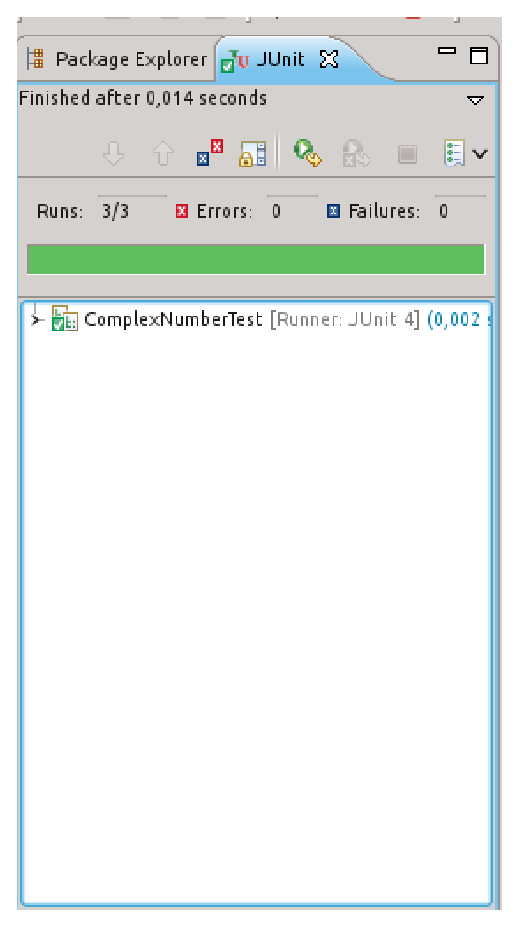
\includegraphics[width=100pt]{./figs/Results}
\end{center}

\end{frame}

%%%%%%%%%%%%%%%%%%%%%%%%%%%%%%%%%%%%%%%%%%%%%%%%%%%%%%%%%%%%%%%%%%%%%%%%%%%%%
%%%%%%%%%%%%%%%%%%%%%%%%%%%%%%%%%%%%%%%%%%%%%%%%%%%%%%%%%%%%%%%%%%%%%%%%%%%%%

\section{Advanced Topics}

%%%%%%%%%%%%%%%%%%%%%%%%%%%%%%%%%%%%%%%%%%%%%%%%%%%%%%%%%%%%%%%%%%%%%%%%%%%%%
%%%%%%%%%%%%%%%%%%%%%%%%%%%%%%%%%%%%%%%%%%%%%%%%%%%%%%%%%%%%%%%%%%%%%%%%%%%%%

\subsection{Testing Suites}

%%%%%%%%%%%%%%%%%%%%%%%%%%%%%%%%%%%%%%%%%%%%%%%%%%%%%%%%%%%%%%%%%%%%%%%%%%%%%

\begin{frame}[fragile]{Suites}

Run different sets of unit tests

Using \texttt{@Suite} annotation

\begin{lstlisting}[language=Java,basicstyle=\scriptsize]  
import org.junit.platform.suite.api.IncludeTags;
import org.junit.platform.suite.api.SelectPackages;
import org.junit.platform.suite.api.Suite;

@SelectPackages({"uah.packageA"
                ,"uah.packageB"})

@IncludeTags("production")
@Suite
public class JUnit5TestSuiteExample {
}
\end{lstlisting}

\end{frame}



%%%%%%%%%%%%%%%%%%%%%%%%%%%%%%%%%%%%%%%%%%%%%%%%%%%%%%%%%%%%%%%%%%%%%%%%%%%%%
%%%%%%%%%%%%%%%%%%%%%%%%%%%%%%%%%%%%%%%%%%%%%%%%%%%%%%%%%%%%%%%%%%%%%%%%%%%%%

\subsection{Testing Exceptions}


%%%%%%%%%%%%%%%%%%%%%%%%%%%%%%%%%%%%%%%%%%%%%%%%%%%%%%%%%%%%%%%%%%%%%%%%%%%%%

\begin{frame}[fragile]{Exceptions}

  The coefficient $a$ must not be zero. Therefore, the following code:
  
  \texttt{instance = new QuadraticEquation(0,1,1);}
  
  will throw an exception when executing:
  
  \texttt{boolean result = instance.checkCoefficientsAreOk();}
  
  This is tested with the annotation \texttt{@Test(expected=CoefficientsException.class)}.
  
  \begin{lstlisting}[language=JAVA,basicstyle=\scriptsize]
      @Test(expected=CoefficientsException.class)
      public void testCheckCoefficientsAreOkException() throws CoefficientsException {
          System.out.println("checkCoefficientsAreOk with Exception raised");
          QuadraticEquation instance;
          instance = new QuadraticEquation(0,1,1);
          boolean result = instance.checkCoefficientsAreOk();
      }
  \end{lstlisting}
  
  \end{frame}


%%%%%%%%%%%%%%%%%%%%%%%%%%%%%%%%%%%%%%%%%%%%%%%%%%%%%%%%%%%%%%%%%%%%%%%%%%%%%
%%%%%%%%%%%%%%%%%%%%%%%%%%%%%%%%%%%%%%%%%%%%%%%%%%%%%%%%%%%%%%%%%%%%%%%%%%%%%
\subsection{Testing Private Methods}

%%%%%%%%%%%%%%%%%%%%%%%%%%%%%%%%%%%%%%%%%%%%%%%%%%%%%%%%%%%%%%%%%%%%%%%%%%%%%

\begin{frame}{Testing Private Methods}

In general private methods are not tested directly (they are tested indirectly through other public methods). However, if there is a need to do there are several alternatives:

\begin{itemize}
 \item Change the visibility (make them public) temporarily. However, this changes the original program and does not follow the criteria of keeping tests and source code independently.
 \item Use Java reflection mechanisms
\end{itemize}


\end{frame}

%%%%%%%%%%%%%%%%%%%%%%%%%%%%%%%%%%%%%%%%%%%%%%%%%%%%%%%%%%%%%%%%%%%%%%%%%%%%%


\begin{frame}[fragile]{Testing Private Methods - Example}

\begin{lstlisting}[language=Java,basicstyle=\tiny]
    public void testComputeDiscriminant() throws Exception {
        System.out.println("checkCoefficientsAreOk");
         Class c = null;
         Object ins = new QuadraticEquation(1,1,1);
         Method m = null;
         c = Class.forName("example.QuadraticEquation");
         m = c.getDeclaredMethod("computeDiscriminant");
         // Remove private access restriction:
         m.setAccessible(true);
         Object res = m.invoke(ins);
         Double result = (Double)res;
         System.out.println(result);
         double expectedResult = -3.0;
         assertEquals(result.doubleValue(), expectedResult);
    }
\end{lstlisting}

\end{frame}

%%%%%%%%%%%%%%%%%%%%%%%%%%%%%%%%%%%%%%%%%%%%%%%%%%%%%%%%%%%%%%%%%%%%%%%%%%%%%
%%%%%%%%%%%%%%%%%%%%%%%%%%%%%%%%%%%%%%%%%%%%%%%%%%%%%%%%%%%%%%%%%%%%%%%%%%%%%

\subsection{Parametrized tests}

%%%%%%%%%%%%%%%%%%%%%%%%%%%%%%%%%%%%%%%%%%%%%%%%%%%%%%%%%%%%%%%%%%%%%%%%%%%%%

\begin{frame}{Parametrized tests}

The parametrized test is an automated test in which the parameters change automatically.

\end{frame}

%%%%%%%%%%%%%%%%%%%%%%%%%%%%%%%%%%%%%%%%%%%%%%%%%%%%%%%%%%%%%%%%%%%%%%%%%%%%%

\begin{frame}[fragile]{Parametrized tests - Example}

\begin{lstlisting}[language=Java,basicstyle=\tiny]
import static org.junit.Assert.assertEquals;
import java.util.Arrays;
import java.util.Collection;
import org.junit.Test;
import org.junit.runner.RunWith;
import org.junit.runners.Parameterized;
import org.junit.runners.Parameterized.Parameters;

//@RunWith(MockitoJUnitRunner.class)
@RunWith(Parameterized.class)
public class QuadraticEquationparTest {
  private QuadraticEquation qe;

  private Double coeficient;

  //Constructor
  public QuadraticEquationparTest(Double coeficient) {
    this.coeficient = coeficient;
  }

  @Parameters //Definition of the parameters.
  public static Collection<Double[]> data() {
    Double[][] data = new Double[][] { {1.0}, {2.0}, {3.0}, {4.0} , {14.0} };
  return Arrays.asList(data);
}
\end{lstlisting}
\end{frame}

%%%%%%%%%%%%%%%%%%%%%%%%%%%%%%%%%%%%%%%%%%%%%%%%%%%%%%%%%%%%%%%%%%%%%%%%%%%%%


\begin{frame}[fragile]
\begin{lstlisting}[language=Java,basicstyle=\tiny]
@Test
public void checkCoefficientsAreOk() throws Exception {
  System.out.println("Coeficients");
  boolean expResult = true;
  qe = new QuadraticEquation(coeficient,6.0,8.0);
  boolean result = qe.checkCoefficientsAreOk();
  assertEquals(expResult, result);
}
\end{lstlisting}
\end{frame}



%%%%%%%%%%%%%%%%%%%%%%%%%%%%%%%%%%%%%%%%%%%%%%%%%%%%%%%%%%%%%%%%%%%%%%%%%%%%%
%%%%%%%%%%%%%%%%%%%%%%%%%%%%%%%%%%%%%%%%%%%%%%%%%%%%%%%%%%%%%%%%%%%%%%%%%%%%%
%%%%%%%%%%%%%%%%%%%%%%%%%%%%%%%%%%%%%%%%%%%%%%%%%%%%%%%%%%%%%%%%%%%%%%%%%%%%%

\section{Testing with Mock Objects}

%%%%%%%%%%%%%%%%%%%%%%%%%%%%%%%%%%%%%%%%%%%%%%%%%%%%%%%%%%%%%%%%%%%%%%%%%%%%%

\subsection{Mock Objects}

%%%%%%%%%%%%%%%%%%%%%%%%%%%%%%%%%%%%%%%%%%%%%%%%%%%%%%%%%%%%%%%%%%%%%%%%%%%

\begin{frame}{What are Mock objects?}


Sometimes tests need to be carried out without having all objects implemented or the instantiation of all needed classes is very expensive (e.g., when dealing with databases)

Advantages of using mock objects include:

\begin{itemize}
 \item Easy to instantiate
 \item If a CUT fails, the failure is located in the CUT, never in the mock!
 \item They allow us to reduce the testing time with simpler and faster classes
\end{itemize}

In Java, well-known frameworks include: Mockito, JMock and Easymock.

\end{frame}

%%%%%%%%%%%%%%%%%%%%%%%%%%%%%%%%%%%%%%%%%%%%%%%%%%%%%%%%%%%%%%%%%%%%%%%%%%%%%

\begin{frame}{Process}

Process to create mock objects

\begin{enumerate}
 \item Create the necessary Mock objects
 \item Define their behaviour, establishing expectations
 \item Create CUT instances using the mock objects
 \item Run the test methods 
 \item Check with the mock objects if expectations were fulfilled. 
\end{enumerate}

\end{frame}


%%%%%%%%%%%%%%%%%%%%%%%%%%%%%%%%%%%%%%%%%%%%%%%%%%%%%%%%%%%%%%%%%%%%%%%%%%%%%

\subsection{Testing with Mockito}


%%%%%%%%%%%%%%%%%%%%%%%%%%%%%%%%%%%%%%%%%%%%%%%%%%%%%%%%%%%%%%%%%%%%%%%%%%%%%

\begin{frame}

''Mockito is a mocking framework that tastes really good. It lets you write beautiful tests with clean \& simple API. Mockito doesn't give you hangover because the tests are very readable and they produce clean verification errors.''


\url{https://site.mockito.org/}

With mock objects and Mockito we can do:

\begin{enumerate}
  \item Test the behaviour
  \item Force the behaviour
  \item Use matchers in arguments passing
  \item Call order verification
  \item Etc.
\end{enumerate}
\end{frame}

%%%%%%%%%%%%%%%%%%%%%%%%%%%%%%%%%%%%%%%%%%%%%%%%%%%%%%%%%%%%%%%%%%%%%%%%%%%%%


\begin{frame}{Installing Mockito}

Mockito is usually used via Maven or Gradle to handle the dependencies.

%\begin{lstlisting}[language=XML,basicstyle=\tiny]
%   <!-- https://mvnrepository.com/artifact/org.mockito/mockito-core -->
%   <dependency>
%       <groupId>org.mockito</groupId>
%       <artifactId>mockito-core</artifactId>
%       <version>4.1.0</version>
%       <scope>test</scope>
%   </dependency>
%\end{lstlisting}

\url{https://site.mockito.org/}

Manually, it is always possible to include the \texttt{.jar} file into your project.

\end{frame}




%%%%%%%%%%%%%%%%%%%%%%%%%%%%%%%%%%%%%%%%%%%%%%%%%%%%%%%%%%%%%%%%%%%%%%%%%%%%%%%

\begin{frame}[fragile]{Summary}

JUnit is a must in software engineering. 

It can be used in combination with other frameworks such as Mockito, EasyMock, etc.

It should be part of the software development life cycle with:
\begin{itemize}
  \item Continuous integration
  \item Configuration management, e.g., Git.
  \item etc.
\end{itemize}

\end{frame}


%%%%%%%%%%%%%%%%%%%%%%%%%%%%%%%%%%%%%%%%%%%%%%%%%%%%%%%%%%%%%%%%%%%%%%%%%%%%%%%

\end{document} 
























% %%%%%%%%%%%%%%%%%%%%%%%%%%%%%%%%%%%%%%%%%%%%%%%%%%%%%%%%%%%%%%%%%%%%%%%%%%%%%
% Example:



% \begin{frame}[fragile]

% \begin{lstlisting}[language=Java,basicstyle=\tiny]
% public class QuadraticEquation {

%     /* quadratic coefficient */
%     private double a =  0;
%     /* linear coefficient */
%     private double b = 0;
%     /* free term */
%     private double c = 0;

%     /**
%      * Creates the quadratic equation from its parameters.
%      */
%     public QuadraticEquation(double a, double b, double c){
%         this.a = a; this.b = b; this.c = c;
%     }

%     /**
%      * Helper method to check the coefficients are ok.
%      */
%     protected boolean checkCoefficientsAreOk() throws Exception{
%         if (a == 0) throw new Exception();
%         return true;
%     }

%     /**
%      *  Computes the discriminant of the equation.
%      */
%     private double computeDiscriminant(){
%         return b*b - 4*a*c;
%     }

% \end{lstlisting}
% \end{frame}

% %%%%%%%%%%%%%%%%%%%%%%%%%%%%%%%%%%%%%%%%%%%%%%%%%%%%%%%%%%%%%%%%%%%%%%%%%%%%%

% \begin{frame}[fragile]


% \begin{lstlisting}[language=Java,basicstyle=\tiny]
%   /**
%      * Get solutions of the equation.
%      * The method returns:
%      * (a) Either two real or two imaginary solutions
%      * in positions 0 and 1 of the array
%      * (b) A single solution in position 0 of the array with the other
%      * set to null.
%      */
%     public ComplexNumber[] getSolutions(){
%         // This check is defensive programming, as the contract of
%         // the class makes clear a should not be zero.
%     	try
%     	{
%     	if (!checkCoefficientsAreOk())
%             return null;
%     	}catch(Exception e)
%     	{
%     		System.out.println(e.toString());
%     	}
%         Double disc = computeDiscriminant();
%         ComplexNumber[] result = new ComplexNumber[2];
%         if (disc == 0){
%             Double sol = - (b/(2*a));
%             result[0] = new ComplexNumber(sol, 0.0);
%         }else if (disc > 0){
%             Double sol1 = (-b + Math.sqrt(disc))/(2*a);
%             result[0] = new ComplexNumber(sol1, 0.0);

% \end{lstlisting}
% \end{frame}

% % %%%%%%%%%%%%%%%%%%%%%%%%%%%%%%%%%%%%%%%%%%%%%%%%%%%%%%%%%%%%%%%%%%%%%%%%%%%%%

% \begin{frame}[fragile]

% \begin{lstlisting}[language=JAVA,basicstyle=\tiny]

%             result[0] = new ComplexNumber(sol1, 0.0);
%             Double sol2 = (-b - Math.sqrt(disc))/(2*a);
%             result[1] = new ComplexNumber(sol2, 0.0);
%         }
%         else{
%             Double realPart = -b/(2*a);
%             Double imagPart = disc/(2*a);
%             result[0] = new ComplexNumber(realPart, imagPart);
%             result[1] = new ComplexNumber(realPart, -imagPart);
%         }
%         return result;
%     }

%    }
% \end{lstlisting}
% \end{frame}

% %%%%%%%%%%%%%%%%%%%%%%%%%%%%%%%%%%%%%%%%%%%%%%%%%%%%%%%%%%%%%%%%%%%%%%%%%%%%%

% % \begin{frame}

% % First step is to create JUnit test classes as usual.

% % Then create the test methods.

% % \end{frame}

% %%%%%%%%%%%%%%%%%%%%%%%%%%%%%%%%%%%%%%%%%%%%%%%%%%%%%%%%%%%%%%%%%%%%%%%%%%%%%

% \begin{frame}[fragile]
% \begin{lstlisting}[language=JAVA,basicstyle=\tiny]
% import static org.junit.Assert.*;
% import java.util.Arrays;
% import org.junit.After;
% import org.junit.Before;
% import org.junit.Test;

% //@RunWith(MockitoJUnitRunner.class)
% public class QuadraticEquationTest
% {
% 	 private QuadraticEquation qe;
% 	 private QuadraticEquation qe1;
	
% 	@Before
% 	public void setUp() throws Exception
% 	{
% 		qe = new QuadraticEquation(1.0, 5.0, 0.0);
% 		qe1 = new QuadraticEquation(0.0, 5.0, 0.0);
% 	}

% 	@After
% 	public void tearDown() throws Exception
% 	{
% 		qe = new QuadraticEquation(0.0, 0.0, 0.0);
% 	}
% \end{lstlisting}
% \end{frame}

% %%%%%%%%%%%%%%%%%%%%%%%%%%%%%%%%%%%%%%%%%%%%%%%%%%%%%%%%%%%%%%%%%%%%%%%%%%%%%

% \begin{frame}[fragile]
% \begin{lstlisting}[language=JAVA,basicstyle=\tiny]
% 	@Test
% 	public void checkCoefficientsAreOk() throws Exception {
% 		System.out.println("Coeficients");
% 		boolean expResult = true;
% 		boolean result = qe.checkCoefficientsAreOk();
% 		assertEquals(expResult, result);
% 	}

%   //Testing exceptions the first coeficient must not be 0
% 	@Test(expected = Exception.class) 
% 	public void checkCoefficientsAreOk1() throws Exception {
% 		System.out.println("Coeficients");
% 		boolean expResult = true;
% 		boolean result = qe1.checkCoefficientsAreOk();
% 		assertEquals(expResult, result);
% 	}
	
% 	@Test
% 	public void getSolutions() throws Exception {
% 		System.out.println("Solutions");
% 		ComplexNumber[] expected = { new ComplexNumber(0.0, 0.0),
% 				new ComplexNumber(-5.0, 0.0) };
% 		ComplexNumber[] result = qe.getSolutions();
% 		System.out.println(Arrays.equals(result, expected));
% 		assertArrayEquals(expected, result);
% 	}}
% \end{lstlisting}
% \end{frame}

% %%%%%%%%%%%%%%%%%%%%%%%%%%%%%%%%%%%%%%%%%%%%%%%%%%%%%%%%%%%%%%%%%%%%%%%%%%%%%

% \begin{frame}
% Now we going to do the same with the \texttt{ComplexNumbers}.
% \end{frame}

% %%%%%%%%%%%%%%%%%%%%%%%%%%%%%%%%%%%%%%%%%%%%%%%%%%%%%%%%%%%%%%%%%%%%%%%%%%%%%

% \begin{frame}[fragile]{Example}
% \begin{lstlisting}[language=JAVA,basicstyle=\tiny]
% class ComplexNumber {
%     private Double realPart;
%     private Double imagPart;

%     /**
%      * Construct a new ComplexNumber that has the value 0 + 0i.
%      */
%     public ComplexNumber() {
%     }

%     /**
%      * Construct a new ComplexNumber with the value realPart + 0i.
%      *
%      * @param realPart initial value for the real part
%      */
%     public ComplexNumber(Double realPart) {
% 	      this.realPart = realPart;
%     }

%     /**
%      * Construct a new ComplexNumber
%      *
%      * @param realPart initial value for the real part
%      * @param imagPart initial value for the imaginary part
%      */
%     public ComplexNumber(Double realPart, Double imagPart) {
% 	    this.realPart = realPart;
% 	    this.imagPart = imagPart;
%     }
% \end{lstlisting}
% \end{frame}


% %%%%%%%%%%%%%%%%%%%%%%%%%%%%%%%%%%%%%%%%%%%%%%%%%%%%%%%%%%%%%%%%%%%%%%%%%%%%%

% \begin{frame}[fragile]
% \begin{lstlisting}[language=JAVA,basicstyle=\tiny]
%     /**
%      * Test whether the this ComplexNumber and the ComplexNumber theNum
%      * are equal.  Two ComplexNumbers are equal if their
%      * real parts are equal and their imaginary parts are equal.
%      *
%      * @param theNum the ComplexNumber to which this ComplexNumber is
%      *               to be compared for equality.
%      * @return true if the real and imaginary parts of this
%      *         ComplexNumber are equal to the real and imaginary
%      *         parts of theNum, and false otherwise.
%      */
%     public boolean equals(ComplexNumber theNum) {
% 	    return ((realPart == theNum.realPart) &&
% 		          (imagPart == theNum.imagPart));
%     }
% \end{lstlisting}
% \end{frame}

% %%%%%%%%%%%%%%%%%%%%%%%%%%%%%%%%%%%%%%%%%%%%%%%%%%%%%%%%%%%%%%%%%%%%%%%%%%%%%

% \begin{frame}[fragile]
% \begin{lstlisting}[language=Java,basicstyle=\tiny]
%   /**
%      * Return a reference to a new ComplexNumber with value equal
%      * to the sum of this ComplexNumber and the ComplexNumber theNum.
%      *
%      * @param theNum a ComplexNumber to be added to this ComplexNumber.
%      * @return a reference to a new ComplexNumber equal to the sum of this
%      *         ComplexNumber and theNum.
%      */
%     public ComplexNumber add(ComplexNumber theNum) {
% 	    return new ComplexNumber(realPart + theNum.realPart,
% 				                       imagPart + theNum.imagPart);
%     }

%     /**
%      * Return a reference to a new ComplexNumber with value equal
%      * to the difference between this ComplexNumber and the
%      * ComplexNumber theNum.
%      *
%      * @param theNum a ComplexNumber to be subtracted from this ComplexNumber.
%      * @return a reference to a new ComplexNumber equal to the difference
%      *         between this ComplexNumber and theNum.
%      */
%     public ComplexNumber subtract(ComplexNumber theNum) {
% 	    return new ComplexNumber(realPart - theNum.realPart,
% 				                       imagPart - theNum.imagPart);
%     }

% \end{lstlisting}
% \end{frame}

% %%%%%%%%%%%%%%%%%%%%%%%%%%%%%%%%%%%%%%%%%%%%%%%%%%%%%%%%%%%%%%%%%%%%%%%%%%%%%


% \begin{frame}[fragile]
% \begin{lstlisting}[language=JAVA,basicstyle=\tiny]
%     /**
%      * Get the real part of this ComplexNumber.
%      *
%      * @return the real part of this ComplexNumber.
%      */
%     public Double getRealPart() {
% 	     return realPart;
%     }

%     /**
%      * Get the imaginary part of this ComplexNumber.
%      *
%      * @return the imaginary part of this ComplexNumber.
%      */
%     public Double getImaginaryPart() {
% 	    return imagPart;
%     }

%     /**
%      * Convert this ComplexNumber into a String representation.
%      *
%      * @return a String representation of this ComplexNumber.
%      */
%     @Override
%     public String toString() {
% 	    // If the imagPart is >= 0 print out a + b i
% 	    if (imagPart >= 0) {
% 	      return realPart + " + " + imagPart + " i";
%     	}
% 	    // If the imagPart is < 0 print out a - b i
% 	    else {
% 	      return realPart + " - " + (-imagPart) + " i";
% 	    }
%     }
% }
% \end{lstlisting}
% \end{frame}

% %%%%%%%%%%%%%%%%%%%%%%%%%%%%%%%%%%%%%%%%%%%%%%%%%%%%%%%%%%%%%%%%%%%%%%%%%%%%%

% \begin{frame}[fragile]
% \begin{lstlisting}[language=JAVA,basicstyle=\tiny]
% import static org.junit.Assert.*;
% import static org.mockito.Mockito.*;
% import org.junit.Before;
% import org.junit.Test;

% public class ComplexNumberTest{
% 	private ComplexNumber cZero ;
% 	private ComplexNumber cOneZero ;
% 	private ComplexNumber cZeroOne ;
% 	private ComplexNumber cOneOne ;
	
% 	@Before
% 	public void setUp() throws Exception {
% 		cZero = new ComplexNumber(0.0,0.0) ;
% 		cOneZero = new ComplexNumber(1.0,0.0) ;
% 		cZeroOne = new ComplexNumber(0.0,1.0) ;
% 		cOneOne = new ComplexNumber (1.0,1.0) ;
% 	}
% \end{lstlisting}
% \end{frame}

% %%%%%%%%%%%%%%%%%%%%%%%%%%%%%%%%%%%%%%%%%%%%%%%%%%%%%%%%%%%%%%%%%%%%%%%%%%%%%

% \begin{frame}[fragile]

% \begin{lstlisting}[language=Java,basicstyle=\tiny]
% 	@Test
% 	public void equals() throws Exception {
% 		System.out.println("equals");
% 		boolean expResult = true ;
% 		boolean result = cOneZero.equals(cOneZero);
% 		assertEquals(expResult,result);
% 	}

% 	@Test
% 	public void add() throws Exception {
% 		System.out.println("add");
% 		ComplexNumber result = cZeroOne.add(cOneZero);
% 		assertEquals(cOneOne.toString(),result.toString());
% 	}

% 	@Test
% 	public void subtract() throws Exception	{
% 		System.out.println("sub");
% 		ComplexNumber result = cOneZero.subtract(cOneZero);
% 		assertEquals(cZero.toString(),result.toString());
% 	}
% \end{lstlisting}

% \end{frame}

% %%%%%%%%%%%%%%%%%%%%%%%%%%%%%%%%%%%%%%%%%%%%%%%%%%%%%%%%%%%%%%%%%%%%%%%%%%%%%

% \begin{frame}[fragile]

% \begin{lstlisting}[language=JAVA,basicstyle=\scriptsize]
%   @Test public void getRealPart() throws Exception {
%     System.out.println("getReal") ;
%     double expResult = 0.0 ;
%     double result = cZeroOne.getRealPart( ) ;
%     assertEquals(expResult,result,0.1) ;
%   }
%   @Test public void getImaginaryPart() throws Exception {
%     System.out.println("getImg") ;
%     double expResult = 1.0;
%     double result = cZeroOne.getImaginaryPart();
%     assertEquals(expResult,result,0.1) ;
%   }
%   @Test public void getImaginaryPart2() throws Exception {
%     System.out.println( "getImg" ) ;
%     ComplexNumber cNumber = mock(ComplexNumber.class);
%     when(cNumber.getImaginaryPart()).thenReturn(1.0);
%     double expResult = 1.0;
%     double result = cZeroOne.getImaginaryPart();
%     assertEquals(expResult,result,0.1) ;
%   }
% \end{lstlisting
  


% %%%%%%%%%%%%%%%%%%%%%%%%%%%%%%%%%%%%%%%%%%%%%%%%%%%%%%%%%%%%%%%%%%%%%%%%%%%%%

% \section{First Example}

% %%%%%%%%%%%%%%%%%%%%%%%%%%%%%%%%%%%%%%%%%%%%%%%%%%%%%%%%%%%%%%%%%%%%%%%%%%%%%


% \begin{frame}[fragile]{\texttt{ComplexNumber} class -- Class Under Test (CUT)}

% We will use \texttt{ComplexNumber} class and later this class will be used to calculate quadratic equations.

% The structure of \texttt{ComplexNumber} is as follows:

% \begin{center}
%  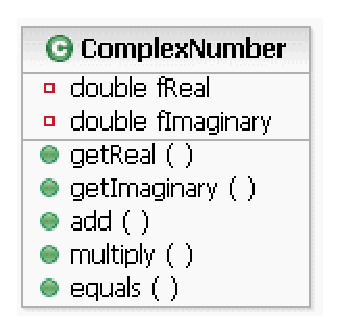
\includegraphics[width=75pt]{./figs/ComplexNumber}
% \end{center}

% And the operations are as follows:

% \begin{itemize}
%  \item Addition: $(a,b)+(c,d)=(a+c)+(b+d)i$
%  \item Multiplication: $(a,b)\cdot(c,d)=(ac-bd) + (ad+cb)i$
%  \item Equality: $(a,b)=(c,d) \Leftrightarrow a=c \wedge b=d$
% \end{itemize}

% \end{frame}


% %%%%%%%%%%%%%%%%%%%%%%%%%%%%%%%%%%%%%%%%%%%%%%%%%%%%%%%%%%%%%%%%%%%%%%%%%%%%%


% \begin{frame}[fragile]{\texttt{ComplexNumber} class -- CUT I}


% \begin{lstlisting}[language=Java,basicstyle=\scriptsize]
% public class ComplexNumber {
%     private double fReal;
%     private double fImaginary;

%   public ComplexNumber(double re, double im) {
%     fReal = re;
%     fImaginary = im;
%   }

%   public double getReal() {
%     return fReal;
%   }

%   public double getImaginary() {
%     return fImaginary;
%   }
% }

% public ComplexNumber add(ComplexNumber c) {
%   return new ComplexNumber(getReal() + c.getReal(), getImaginary() + c.getImaginary());
% }
% \end{lstlisting}

% \end{frame}

% % %%%%%%%%%%%%%%%%%%%%%%%%%%%%%%%%%%%%%%%%%%%%%%%%%%%%%%%%%%%%%%%%%%%%%%%%%%%%%

% \begin{frame}[fragile]{\texttt{ComplexNumber} class -- CUT II}

% \begin{lstlisting}[language=Java,basicstyle=\scriptsize]
% public ComplexNumber multiply(ComplexNumber c) {
%   double re = getReal() * c.getReal() - getImaginary() * c.getImaginary();
%   double im = getImaginary() * c.getReal() + getReal() * c.getImaginary();
%   return new ComplexNumber(re, im);
% }

% @Override
% public boolean equals(Object anObject) {
%   if (anObject instanceof ComplexNumber) {
%     ComplexNumber c = (ComplexNumber) anObject;
%     return ((c.getReal() == getReal()) && (c.getImaginary() == getImaginary()));
%   } else
%     return false;
%   }
% }
% \end{lstlisting}

% \end{frame}




% %%%%%%%%%%%%%%%%%%%%%%%%%%%%%%%%%%%%%%%%%%%%%%%%%%%%%%%%%%%%%%%%%%%%%%%%%%%%%
% %%%%%%%%%%%%%%%%%%%%%%%%%%%%%%%%%%%%%%%%%%%%%%%%%%%%%%%%%%%%%%%%%%%%%%%%%%%%%

% \subsection{Testing Suites}

% %%%%%%%%%%%%%%%%%%%%%%%%%%%%%%%%%%%%%%%%%%%%%%%%%%%%%%%%%%%%%%%%%%%%%%%%%%%%%

% % \begin{frame}[fragile]{Suites}

% %   Run different sets of unit tests

% %   Using \texttt{@Suite} annotation

% %   % \begin{lstlisting}[language=Java,basicstyle=\tiny]  
% %   % import org.junit.platform.suite.api.IncludeTags;
% %   % import org.junit.platform.suite.api.SelectPackages;
% %   % import org.junit.platform.suite.api.Suite  % \begin{lstlisting}[language=Java,basicstyle=\tiny]  
% %   % import org.junit.platform.suite.api.IncludeTags;
% %   % import org.junit.platform.suite.api.SelectPackages;
% %   % import org.junit.platform.suite.api.Suite;
  
% %   % @SelectPackages({"uah.packageA"
% %   %                 ,"uah.packageB"})
  
% %   % @IncludeTags("production")
% %   % @Suite
% %   % public class JUnit5TestSuiteExample {
% %   % }
% %   % \end
% %   % \end{lstlisting};
  
% %   % @SelectPackages({"uah.packageA"
% %   %                 ,"uah.packageB"})
  
% %   % @IncludeTags("production")
% %   % @Suite
% %   % public class JUnit5TestSuiteExample {
% %   % }
% %   % \end
% %   % \end{lstlisting}

% % \end{frame}

% %%%%%%%%%%%%%%%%%%%%%%%%%%%%%%%%%%%%%%%%%%%%%%%%%%%%%%%%%%%%%%%%%%%%%%%%%%%%%
% %%%%%%%%%%%%%%%%%%%%%%%%%%%%%%%%%%%%%%%%%%%%%%%%%%%%%%%%%%%%%%%%%%%%%%%%%%%%%

% \subsection{Testing Exceptions}


% %%%%%%%%%%%%%%%%%%%%%%%%%%%%%%%%%%%%%%%%%%%%%%%%%%%%%%%%%%%%%%%%%%%%%%%%%%%%%

% \begin{frame}[fragile]{Exceptions}

% The coefficient $a$ must not be zero. Therefore,

% \texttt{instance = new QuadraticEquation(0,1,1);}

% will throw an exception when:

% \texttt{boolean result = instance.checkCoefficientsAreOk();}

% This is tested with:
%     @Test(expected=CoefficientsException.class)

% \begin{lstlisting}[language=JAVA,basicstyle=\scriptsize]
%     @Test(expected=CoefficientsException.class)
%     public void testCheckCoefficientsAreOkException() throws CoefficientsException {
%         System.out.println("checkCoefficientsAreOk with Exception raised");
%         QuadraticEquation instance;
%         instance = new QuadraticEquation(0,1,1);
%         boolean result = instance.checkCoefficientsAreOk();
%     }
% \end{lstlisting}

% \end{frame}



% %%%%%%%%%%%%%%%%%%%%%%%%%%%%%%%%%%%%%%%%%%%%%%%%%%%%%%%%%%%%%%%%%%%%%%%%%%%%%
% %%%%%%%%%%%%%%%%%%%%%%%%%%%%%%%%%%%%%%%%%%%%%%%%%%%%%%%%%%%%%%%%%%%%%%%%%%%%%

% \subsection{Testing Private Methods}

% %%%%%%%%%%%%%%%%%%%%%%%%%%%%%%%%%%%%%%%%%%%%%%%%%%%%%%%%%%%%%%%%%%%%%%%%%%%%%

% \begin{frame}{Testing Private Methods}

% In general private methods are not tested directly (they are tested indirectly through other public methods). However, if there is a need to do there are several alternatives:

% \begin{itemize}
%  \item Change the visibility (make them public) temporarily. However, this changes the original program and does not follow the criteria of keeping tests and source code independently.
%  \item Use Java reflection mechanisms
% \end{itemize}


% \end{frame}

% %%%%%%%%%%%%%%%%%%%%%%%%%%%%%%%%%%%%%%%%%%%%%%%%%%%%%%%%%%%%%%%%%%%%%%%%%%%%%

% \section{Advanced Issues}

% %%%%%%%%%%%%%%%%%%%%%%%%%%%%%%%%%%%%%%%%%%%%%%%%%%%%%%%%%%%%%%%%%%%%%%%%%%%%%

% \subsection{Testing private methods}

% %%%%%%%%%%%%%%%%%%%%%%%%%%%%%%%%%%%%%%%%%%%%%%%%%%%%%%%%%%%%%%%%%%%%%%%%%%%%%


% \begin{frame}[fragile]{Testing Private Methods - Example}

% \begin{lstlisting}[language=Java,basicstyle=\tiny]
%     public void testComputeDiscriminant() throws Exception {
%         System.out.println("checkCoefficientsAreOk");
%          Class c = null;
%          Object ins = new QuadraticEquation(1,1,1);
%          Method m = null;
%          c = Class.forName("example.QuadraticEquation");
%          m = c.getDeclaredMethod("computeDiscriminant");
%          // Remove private access restriction:
%          m.setAccessible(true);
%          Object res = m.invoke(ins);
%          Double result = (Double)res;
%          System.out.println(result);
%          double expectedResult = -3.0;
%          assertEquals(result.doubleValue(), expectedResult);
%     }
% \end{lstlisting}

% \end{frame}

% %%%%%%%%%%%%%%%%%%%%%%%%%%%%%%%%%%%%%%%%%%%%%%%%%%%%%%%%%%%%%%%%%%%%%%%%%%%%%
% %%%%%%%%%%%%%%%%%%%%%%%%%%%%%%%%%%%%%%%%%%%%%%%%%%%%%%%%%%%%%%%%%%%%%%%%%%%%%

% \subsection{Parametrized tests}

% %%%%%%%%%%%%%%%%%%%%%%%%%%%%%%%%%%%%%%%%%%%%%%%%%%%%%%%%%%%%%%%%%%%%%%%%%%%%%

% \begin{frame}{Parametrized tests}

% The parametrized test is an automated test in which the parameters change automatically.

% \end{frame}

% %%%%%%%%%%%%%%%%%%%%%%%%%%%%%%%%%%%%%%%%%%%%%%%%%%%%%%%%%%%%%%%%%%%%%%%%%%%%%

% \begin{frame}[fragile]{Parametrized tests - Example}

% \begin{lstlisting}[language=Java,basicstyle=\tiny]
% import static org.junit.Assert.assertEquals;
% import java.util.Arrays;
% import java.util.Collection;
% import org.junit.Test;
% import org.junit.runner.RunWith;
% import org.junit.runners.Parameterized;
% import org.junit.runners.Parameterized.Parameters;

% //@RunWith(MockitoJUnitRunner.class)
% @RunWith(Parameterized.class)
% public class QuadraticEquationparTest {
%   private QuadraticEquation qe;

%   private Double coeficient;

%   //Constructor
%   public QuadraticEquationparTest(Double coeficient) {
%     this.coeficient = coeficient;
%   }

%   @Parameters //Definition of the parameters.
%   public static Collection<Double[]> data() {
%     Double[][] data = new Double[][] { {1.0}, {2.0}, {3.0}, {4.0} , {14.0} };
%   return Arrays.asList(data);
% }
% \end{lstlisting}
% \end{frame}

% %%%%%%%%%%%%%%%%%%%%%%%%%%%%%%%%%%%%%%%%%%%%%%%%%%%%%%%%%%%%%%%%%%%%%%%%%%%%%


% \begin{frame}[fragile]
% \begin{lstlisting}[language=Java,basicstyle=\tiny]
% @Test
% public void checkCoefficientsAreOk() throws Exception {
%   System.out.println("Coeficients");
%   boolean expResult = true;
%   qe = new QuadraticEquation(coeficient,6.0,8.0);
%   boolean result = qe.checkCoefficientsAreOk();
%   assertEquals(expResult, result);
% }
% \end{lstlisting}
% \end{frame}



% %%%%%%%%%%%%%%%%%%%%%%%%%%%%%%%%%%%%%%%%%%%%%%%%%%%%%%%%%%%%%%%%%%%%%%%%%%%%%
% %%%%%%%%%%%%%%%%%%%%%%%%%%%%%%%%%%%%%%%%%%%%%%%%%%%%%%%%%%%%%%%%%%%%%%%%%%%%%


% \section{Testing with Mock Objects}

% %%%%%%%%%%%%%%%%%%%%%%%%%%%%%%%%%%%%%%%%%%%%%%%%%%%%%%%%%%%%%%%%%%%%%%%%%%%%%

% \subsection{Mock Objects}

% %%%%%%%%%%%%%%%%%%%%%%%%%%%%%%%%%%%%%%%%%%%%%%%%%%%%%%%%%%%%%%%%%%%%%%%%%%%

% \begin{frame}{What are Mock objects?}


% Sometimes tests need to be carried out without having all objects implemented or the instantiation of all needed classes is very expensive (e.g., when dealing with databases)

% Advantages of using mock objects include:

% \begin{itemize}
%  \item Easy to instantiate
%  \item If a CUT fails, the failure is located in the CUT, never in the mock!
%  \item They allow us to reduce the testing time with simpler and faster classes
% \end{itemize}

% In Java, well-known frameworks include: Mockito, JMock and Easymock.

% \end{frame}

% %%%%%%%%%%%%%%%%%%%%%%%%%%%%%%%%%%%%%%%%%%%%%%%%%%%%%%%%%%%%%%%%%%%%%%%%%%%%%

% \begin{frame}{Process}

% Process to create mock objects

% \begin{enumerate}
%  \item Create the necessary Mock objects
%  \item Define their behaviour, establishing expectations
%  \item Create CUT instances using the mock objects
%  \item Run the test methods 
%  \item Check with the mock objects if expectations were fulfilled. 
% \end{enumerate}

% \end{frame}


% %%%%%%%%%%%%%%%%%%%%%%%%%%%%%%%%%%%%%%%%%%%%%%%%%%%%%%%%%%%%%%%%%%%%%%%%%%%%%

% \subsection{Testing with Mockito}


% %%%%%%%%%%%%%%%%%%%%%%%%%%%%%%%%%%%%%%%%%%%%%%%%%%%%%%%%%%%%%%%%%%%%%%%%%%%%%

% \begin{frame}

% ''Mockito is a mocking framework that tastes really good. It lets you write beautiful tests with clean \& simple API. Mockito doesn't give you hangover because the tests are very readable and they produce clean verification errors.''

% Web: \texttt{https://site.mockito.org/}
% \end{frame}

% %%%%%%%%%%%%%%%%%%%%%%%%%%%%%%%%%%%%%%%%%%%%%%%%%%%%%%%%%%%%%%%%%%%%%%%%%%%%

% \begin{frame}[fragile]
% With Mockito we can use mock objects in unit tests to test classes simulating their behaviour with mock objects.

% Some internet examples:

% \begin{lstlisting}[language=Java,basicstyle=\tiny]
% public class MyServiceTest extends UnitilsJUnit4 {
%     private Mock<MyService> myServiceMock;
% }

% @Before
% public void initialize() {
%     myServiceMock = new MockObject<MyService>(MyService.class, this);
% }
% \end{lstlisting}
% \end{frame}

% %%%%%%%%%%%%%%%%%%%%%%%%%%%%%%%%%%%%%%%%%%%%%%%%%%%%%%%%%%%%%%%%%%%%%%%%%%%%

% \begin{frame}
% With mock objects and Mockito we can do:

%   \begin{enumerate}
%   \item Test the behaviour
%   \item Force the behaviour
%   \item Use matchers in arguments passing
%   \item Call order verification
%   \item Etc.
%   \end{enumerate}
% \end{frame}

% %%%%%%%%%%%%%%%%%%%%%%%%%%%%%%%%%%%%%%%%%%%%%%%%%%%%%%%%%%%%%%%%%%%%%%%%%%%%%


% \begin{frame}{Installing Mockito}

% Download Mockito:

% \texttt{\url{https://site.mockito.org/}}

% and include the \texttt{.jar} file into your project.

% ~

% Or use Maven or Gradle to handle the dependencies.

% \end{frame}

% %%%%%%%%%%%%%%%%%%%%%%%%%%%%%%%%%%%%%%%%%%%%%%%%%%%%%%%%%%%%%%%%%%%%%%%%%%%%%

% % \begin{frame}

% % The process is similar as in JUnit:
% % \begin{enumerate}
% %  \item Open the project properties
% %  \item Click on Java Build Path
% %  \item Select the Libraries tab
% %  \item Click the Add External \texttt{.jar} button
% %  \item Choose your mockito \texttt{.jar} library.
% % \end{enumerate}

% % \end{frame}


% %%%%%%%%%%%%%%%%%%%%%%%%%%%%%%%%%%%%%%%%%%%%%%%%%%%%%%%%%%%%%%%%%%%%%%%%%%%%%

% \begin{frame}[fragile]

% \begin{lstlisting}[language=Java,basicstyle=\tiny]
% public class QuadraticEquation {

%     /* quadratic coefficient */
%     private double a =  0;
%     /* linear coefficient */
%     private double b = 0;
%     /* free term */
%     private double c = 0;

%     /**
%      * Creates the quadratic equation from its parameters.
%      */
%     public QuadraticEquation(double a, double b, double c){
%         this.a = a; this.b = b; this.c = c;
%     }

%     /**
%      * Helper method to check the coefficients are ok.
%      */
%     protected boolean checkCoefficientsAreOk() throws Exception{
%         if (a == 0) throw new Exception();
%         return true;
%     }

%     /**
%      *  Computes the discriminant of the equation.
%      */
%     private double computeDiscriminant(){
%         return b*b - 4*a*c;
%     }

% \end{lstlisting}
% \end{frame}

% %%%%%%%%%%%%%%%%%%%%%%%%%%%%%%%%%%%%%%%%%%%%%%%%%%%%%%%%%%%%%%%%%%%%%%%%%%%%%

% \begin{frame}[fragile]


% \begin{lstlisting}[language=Java,basicstyle=\tiny]
%   /**
%      * Get solutions of the equation.
%      * The method returns:
%      * (a) Either two real or two imaginary solutions
%      * in positions 0 and 1 of the array
%      * (b) A single solution in position 0 of the array with the other
%      * set to null.
%      */
%     public ComplexNumber[] getSolutions(){
%         // This check is defensive programming, as the contract of
%         // the class makes clear a should not be zero.
%     	try
%     	{
%     	if (!checkCoefficientsAreOk())
%             return null;
%     	}catch(Exception e)
%     	{
%     		System.out.println(e.toString());
%     	}
%         Double disc = computeDiscriminant();
%         ComplexNumber[] result = new ComplexNumber[2];
%         if (disc == 0){
%             Double sol = - (b/(2*a));
%             result[0] = new ComplexNumber(sol, 0.0);
%         }else if (disc > 0){
%             Double sol1 = (-b + Math.sqrt(disc))/(2*a);
%             result[0] = new ComplexNumber(sol1, 0.0);

% \end{lstlisting}
% \end{frame}

% % %%%%%%%%%%%%%%%%%%%%%%%%%%%%%%%%%%%%%%%%%%%%%%%%%%%%%%%%%%%%%%%%%%%%%%%%%%%%%

% \begin{frame}[fragile]

% \begin{lstlisting}[language=JAVA,basicstyle=\tiny]

%             result[0] = new ComplexNumber(sol1, 0.0);
%             Double sol2 = (-b - Math.sqrt(disc))/(2*a);
%             result[1] = new ComplexNumber(sol2, 0.0);
%         }
%         else{
%             Double realPart = -b/(2*a);
%             Double imagPart = disc/(2*a);
%             result[0] = new ComplexNumber(realPart, imagPart);
%             result[1] = new ComplexNumber(realPart, -imagPart);
%         }
%         return result;
%     }

%    }
% \end{lstlisting}
% \end{frame}

% %%%%%%%%%%%%%%%%%%%%%%%%%%%%%%%%%%%%%%%%%%%%%%%%%%%%%%%%%%%%%%%%%%%%%%%%%%%%%

% % \begin{frame}

% % First step is to create JUnit test classes as usual.

% % Then create the test methods.

% % \end{frame}

% %%%%%%%%%%%%%%%%%%%%%%%%%%%%%%%%%%%%%%%%%%%%%%%%%%%%%%%%%%%%%%%%%%%%%%%%%%%%%

% \begin{frame}[fragile]
% \begin{lstlisting}[language=JAVA,basicstyle=\tiny]
% import static org.junit.Assert.*;
% import java.util.Arrays;
% import org.junit.After;
% import org.junit.Before;
% import org.junit.Test;

% //@RunWith(MockitoJUnitRunner.class)
% public class QuadraticEquationTest
% {
% 	 private QuadraticEquation qe;
% 	 private QuadraticEquation qe1;
	
% 	@Before
% 	public void setUp() throws Exception
% 	{
% 		qe = new QuadraticEquation(1.0, 5.0, 0.0);
% 		qe1 = new QuadraticEquation(0.0, 5.0, 0.0);
% 	}

% 	@After
% 	public void tearDown() throws Exception
% 	{
% 		qe = new QuadraticEquation(0.0, 0.0, 0.0);
% 	}
% \end{lstlisting}
% \end{frame}

% %%%%%%%%%%%%%%%%%%%%%%%%%%%%%%%%%%%%%%%%%%%%%%%%%%%%%%%%%%%%%%%%%%%%%%%%%%%%%

% \begin{frame}[fragile]
% \begin{lstlisting}[language=JAVA,basicstyle=\tiny]
% 	@Test
% 	public void checkCoefficientsAreOk() throws Exception {
% 		System.out.println("Coeficients");
% 		boolean expResult = true;
% 		boolean result = qe.checkCoefficientsAreOk();
% 		assertEquals(expResult, result);
% 	}

%   //Testing exceptions the first coeficient must not be 0
% 	@Test(expected = Exception.class) 
% 	public void checkCoefficientsAreOk1() throws Exception {
% 		System.out.println("Coeficients");
% 		boolean expResult = true;
% 		boolean result = qe1.checkCoefficientsAreOk();
% 		assertEquals(expResult, result);
% 	}
	
% 	@Test
% 	public void getSolutions() throws Exception {
% 		System.out.println("Solutions");
% 		ComplexNumber[] expected = { new ComplexNumber(0.0, 0.0),
% 				new ComplexNumber(-5.0, 0.0) };
% 		ComplexNumber[] result = qe.getSolutions();
% 		System.out.println(Arrays.equals(result, expected));
% 		assertArrayEquals(expected, result);
% 	}}
% \end{lstlisting}
% \end{frame}

% %%%%%%%%%%%%%%%%%%%%%%%%%%%%%%%%%%%%%%%%%%%%%%%%%%%%%%%%%%%%%%%%%%%%%%%%%%%%%

% \begin{frame}
% Now we going to do the same with the \texttt{ComplexNumbers}.
% \end{frame}

% %%%%%%%%%%%%%%%%%%%%%%%%%%%%%%%%%%%%%%%%%%%%%%%%%%%%%%%%%%%%%%%%%%%%%%%%%%%%%

% \begin{frame}[fragile]{Example}
% \begin{lstlisting}[language=JAVA,basicstyle=\tiny]
% class ComplexNumber {
%     private Double realPart;
%     private Double imagPart;

%     /**
%      * Construct a new ComplexNumber that has the value 0 + 0i.
%      */
%     public ComplexNumber() {
%     }

%     /**
%      * Construct a new ComplexNumber with the value realPart + 0i.
%      *
%      * @param realPart initial value for the real part
%      */
%     public ComplexNumber(Double realPart) {
% 	      this.realPart = realPart;
%     }

%     /**
%      * Construct a new ComplexNumber
%      *
%      * @param realPart initial value for the real part
%      * @param imagPart initial value for the imaginary part
%      */
%     public ComplexNumber(Double realPart, Double imagPart) {
% 	    this.realPart = realPart;
% 	    this.imagPart = imagPart;
%     }
% \end{lstlisting}
% \end{frame}


% %%%%%%%%%%%%%%%%%%%%%%%%%%%%%%%%%%%%%%%%%%%%%%%%%%%%%%%%%%%%%%%%%%%%%%%%%%%%%

% \begin{frame}[fragile]
% \begin{lstlisting}[language=JAVA,basicstyle=\tiny]
%     /**
%      * Test whether the this ComplexNumber and the ComplexNumber theNum
%      * are equal.  Two ComplexNumbers are equal if their
%      * real parts are equal and their imaginary parts are equal.
%      *
%      * @param theNum the ComplexNumber to which this ComplexNumber is
%      *               to be compared for equality.
%      * @return true if the real and imaginary parts of this
%      *         ComplexNumber are equal to the real and imaginary
%      *         parts of theNum, and false otherwise.
%      */
%     public boolean equals(ComplexNumber theNum) {
% 	    return ((realPart == theNum.realPart) &&
% 		          (imagPart == theNum.imagPart));
%     }
% \end{lstlisting}
% \end{frame}

% %%%%%%%%%%%%%%%%%%%%%%%%%%%%%%%%%%%%%%%%%%%%%%%%%%%%%%%%%%%%%%%%%%%%%%%%%%%%%

% \begin{frame}[fragile]
% \begin{lstlisting}[language=Java,basicstyle=\tiny]
%   /**
%      * Return a reference to a new ComplexNumber with value equal
%      * to the sum of this ComplexNumber and the ComplexNumber theNum.
%      *
%      * @param theNum a ComplexNumber to be added to this ComplexNumber.
%      * @return a reference to a new ComplexNumber equal to the sum of this
%      *         ComplexNumber and theNum.
%      */
%     public ComplexNumber add(ComplexNumber theNum) {
% 	    return new ComplexNumber(realPart + theNum.realPart,
% 				                       imagPart + theNum.imagPart);
%     }

%     /**
%      * Return a reference to a new ComplexNumber with value equal
%      * to the difference between this ComplexNumber and the
%      * ComplexNumber theNum.
%      *
%      * @param theNum a ComplexNumber to be subtracted from this ComplexNumber.
%      * @return a reference to a new ComplexNumber equal to the difference
%      *         between this ComplexNumber and theNum.
%      */
%     public ComplexNumber subtract(ComplexNumber theNum) {
% 	    return new ComplexNumber(realPart - theNum.realPart,
% 				                       imagPart - theNum.imagPart);
%     }

% \end{lstlisting}
% \end{frame}

% %%%%%%%%%%%%%%%%%%%%%%%%%%%%%%%%%%%%%%%%%%%%%%%%%%%%%%%%%%%%%%%%%%%%%%%%%%%%%


% \begin{frame}[fragile]
% \begin{lstlisting}[language=JAVA,basicstyle=\tiny]
%     /**
%      * Get the real part of this ComplexNumber.
%      *
%      * @return the real part of this ComplexNumber.
%      */
%     public Double getRealPart() {
% 	     return realPart;
%     }

%     /**
%      * Get the imaginary part of this ComplexNumber.
%      *
%      * @return the imaginary part of this ComplexNumber.
%      */
%     public Double getImaginaryPart() {
% 	    return imagPart;
%     }

%     /**
%      * Convert this ComplexNumber into a String representation.
%      *
%      * @return a String representation of this ComplexNumber.
%      */
%     @Override
%     public String toString() {
% 	    // If the imagPart is >= 0 print out a + b i
% 	    if (imagPart >= 0) {
% 	      return realPart + " + " + imagPart + " i";
%     	}
% 	    // If the imagPart is < 0 print out a - b i
% 	    else {
% 	      return realPart + " - " + (-imagPart) + " i";
% 	    }
%     }
% }
% \end{lstlisting}
% \end{frame}

% %%%%%%%%%%%%%%%%%%%%%%%%%%%%%%%%%%%%%%%%%%%%%%%%%%%%%%%%%%%%%%%%%%%%%%%%%%%%%

% \begin{frame}[fragile]
% \begin{lstlisting}[language=JAVA,basicstyle=\tiny]
% import static org.junit.Assert.*;
% import static org.mockito.Mockito.*;
% import org.junit.Before;
% import org.junit.Test;

% public class ComplexNumberTest{
% 	private ComplexNumber cZero ;
% 	private ComplexNumber cOneZero ;
% 	private ComplexNumber cZeroOne ;
% 	private ComplexNumber cOneOne ;
	
% 	@Before
% 	public void setUp() throws Exception {
% 		cZero = new ComplexNumber(0.0,0.0) ;
% 		cOneZero = new ComplexNumber(1.0,0.0) ;
% 		cZeroOne = new ComplexNumber(0.0,1.0) ;
% 		cOneOne = new ComplexNumber (1.0,1.0) ;
% 	}
% \end{lstlisting}
% \end{frame}

% %%%%%%%%%%%%%%%%%%%%%%%%%%%%%%%%%%%%%%%%%%%%%%%%%%%%%%%%%%%%%%%%%%%%%%%%%%%%%

% \begin{frame}[fragile]

% \begin{lstlisting}[language=Java,basicstyle=\tiny]
% 	@Test
% 	public void equals() throws Exception {
% 		System.out.println("equals");
% 		boolean expResult = true ;
% 		boolean result = cOneZero.equals(cOneZero);
% 		assertEquals(expResult,result);
% 	}

% 	@Test
% 	public void add() throws Exception {
% 		System.out.println("add");
% 		ComplexNumber result = cZeroOne.add(cOneZero);
% 		assertEquals(cOneOne.toString(),result.toString());
% 	}

% 	@Test
% 	public void subtract() throws Exception	{
% 		System.out.println("sub");
% 		ComplexNumber result = cOneZero.subtract(cOneZero);
% 		assertEquals(cZero.toString(),result.toString());
% 	}
% \end{lstlisting}

% \end{frame}

% %%%%%%%%%%%%%%%%%%%%%%%%%%%%%%%%%%%%%%%%%%%%%%%%%%%%%%%%%%%%%%%%%%%%%%%%%%%%%

% \begin{frame}[fragile]

% \begin{lstlisting}[language=JAVA,basicstyle=\scriptsize]
%   @Test public void getRealPart() throws Exception {
%     System.out.println("getReal") ;
%     double expResult = 0.0 ;
%     double result = cZeroOne.getRealPart( ) ;
%     assertEquals(expResult,result,0.1) ;
%   }
%   @Test public void getImaginaryPart() throws Exception {
%     System.out.println("getImg") ;
%     double expResult = 1.0;
%     double result = cZeroOne.getImaginaryPart();
%     assertEquals(expResult,result,0.1) ;
%   }
%   @Test public void getImaginaryPart2() throws Exception {
%     System.out.println( "getImg" ) ;
%     ComplexNumber cNumber = mock(ComplexNumber.class);
%     when(cNumber.getImaginaryPart()).thenReturn(1.0);
%     double expResult = 1.0;
%     double result = cZeroOne.getImaginaryPart();
%     assertEquals(expResult,result,0.1) ;
%   }
% \end{lstlisting}

% \end{frame}



%%%%%%%%%%%%%%%%%%%%%%%%%%%%%%%%%%%%%%%%%%%%%%%%%%%%%%%%%%

% \begin{frame}[fragile]

% In this example we are using a Mock to emulate the behaviour of a \texttt{ComplexNumber} type object.

% The \emph{mock} will return  \texttt{1.0} when the \texttt{getImaginaryPart()} method is called.

% \begin{lstlisting}[language=JAVA,basicstyle=\scriptsize]
% @Test
% public void getImaginaryPart2() throws Exception {
%   System.out.println("getImg");
%   ComplexNumber cNumber = mock(ComplexNumber.class); \\Creating the Mock.
%   when(cNumber.getImaginaryPart()).thenReturn(1.0); \\Coding the Mock behaviour.
%   double expResult = 1.0;
%   double result = cZeroOne.getImaginaryPart();
%   assertEquals(expResult,result,0.1) ;
% }
% \end{lstlisting}

% \end{frame}

